\documentclass[11pt]{article}
\input{../shared/project_style.tex}
\rhead{Module 4 Textbook Note}

\begin{document}
\DocTitle{Module 4: Alfv\'en Continuum and Fluid-MHD Eigenmodes}{From magnetic tension to a verified coupled-harmonic eigenvalue benchmark}{Textbook physics note, version 2.0; conventional Python and MATLAB benchmark retained unchanged}

\begin{overviewbox}
\textbf{Textbook note, version 2.0.} This chapter develops the fluid-magnetohydrodynamic description of shear-Alfv\'en waves from the ideal-MHD equations, explains why nonuniform toroidal and stellarator plasmas possess an Alfv\'en continuous spectrum, derives geometric harmonic coupling and spectral gaps, and then constructs the project's verified two-harmonic radial eigenvalue benchmark. The presentation is self-contained enough for a reader with no prior plasma-wave background: every acronym, symbol, approximation, boundary condition, numerical operation, and verification metric is defined. The implemented benchmark remains intentionally reduced. It is a transparent verification target for later kinetic-drive and physics-informed machine-learning modules, not a predictive three-dimensional stellarator stability calculation.
\end{overviewbox}

\ProjectTOC

\section*{Prerequisite basics notes and reading path}
\addcontentsline{toc}{section}{Prerequisite basics notes and reading path}
The chapter rederives its central results, but the standalone basics notes provide slower introductions and additional exercises. The first six entries are completed textbook drafts. Basics 69 and 73 remain explicit scaffolds in the present curriculum, so their numerical material is developed directly and fully in this chapter.

\begin{longtable}{>{\RaggedRight\arraybackslash}p{0.14\textwidth} >{\RaggedRight\arraybackslash}p{0.29\textwidth} >{\RaggedRight\arraybackslash}p{0.47\textwidth}}
\toprule
\textbf{Basics note} & \textbf{Subject} & \textbf{Role in Module 4}\\
\midrule
\endfirsthead
\toprule
\textbf{Basics note} & \textbf{Subject} & \textbf{Role in Module 4}\\
\midrule
\endhead
\href{run:basics/basics_29_linearization_of_mhd_equations.pdf}{Basics 29} & Linearization of MHD equations & Equilibrium-plus-perturbation expansions, first-order equations, normal modes, and the origin of an eigenvalue problem.\\
\href{run:basics/basics_32_alfven_waves_from_first_principles.pdf}{Basics 32} & Alfv\'en waves from first principles & Magnetic tension, shear polarization, the Alfv\'en speed, and the uniform-plasma dispersion relation.\\
\href{run:basics/basics_34_parallel_wave_number_and_field_line_propagation.pdf}{Basics 34} & Parallel wave number and field-line propagation & Fourier conventions, field-line pitch, rotational transform, rational surfaces, and $k_\parallel$.\\
\href{run:basics/basics_35_alfven_continuum.pdf}{Basics 35} & Alfv\'en continuum & Local continuum frequencies, resonant surfaces, phase mixing, and the distinction between a continuum and a discrete spectrum.\\
\href{run:basics/basics_36_coupled_harmonics_and_avoided_crossings.pdf}{Basics 36} & Coupled harmonics and avoided crossings & Two-mode matrices, eigenvalue repulsion, mixing angles, gap formation, and positivity.\\
\href{run:basics/basics_37_toroidal_alfven_eigenmodes.pdf}{Basics 37} & Toroidicity-induced Alfv\'en eigenmodes & Neighboring-harmonic coupling, TAE gaps, global mode localization, and links to energetic-particle physics.\\
\href{run:basics/basics_69_finite_volume_methods.pdf}{Basics 69} & Finite-volume methods & Control-volume integration, face fluxes, conservative radial discretization, and boundary-face treatment.\\
\href{run:basics/basics_73_numerical_eigenvalue_solvers.pdf}{Basics 73} & Numerical eigenvalue solvers & Sparse symmetric matrices, Lanczos iteration, residuals, normalization, orthogonality, and mode tracking.\\
\bottomrule
\caption{Recommended prerequisite path. A focused first reading is 29 $\rightarrow$ 32 $\rightarrow$ 34 $\rightarrow$ 35 $\rightarrow$ 36 $\rightarrow$ 37, followed by the numerical sections of this chapter.}
\label{tab:module4_prerequisites}
\end{longtable}

\begin{notebox}
\textbf{Relationship to Module 1.} Module 1 supplies the equilibrium magnetic geometry, density, magnetic-field strength, rotational transform, flux coordinates, metric coefficients, and boundary surfaces on which a realistic Module 4 calculation would operate. The present benchmark replaces those high-dimensional inputs by analytic radial profiles so that every limiting case and numerical operation can be checked independently.
\end{notebox}

\SymbolsAcronymsSection
\begin{symtable}
AE & Alfv\'en eigenmode & A global shear-Alfv\'en oscillation with a discrete or weakly continuum-coupled frequency.\\
TAE & Toroidicity-induced Alfv\'en eigenmode & An AE associated primarily with toroidal coupling of neighboring poloidal harmonics.\\
EAE & Ellipticity-induced Alfv\'en eigenmode & An AE associated with ellipticity-driven harmonic coupling, commonly involving $\Delta m=2$.\\
HAE & Helicity-induced Alfv\'en eigenmode & An AE produced by helical geometric harmonics, especially relevant in stellarators.\\
NAE & Noncircularity-induced Alfv\'en eigenmode & General name for modes associated with noncircular shaping harmonics.\\
RSAE & Reversed-shear Alfv\'en eigenmode & A mode localized near a minimum or maximum of the safety-factor or rotational-transform profile.\\
MHD & Magnetohydrodynamics & A continuum-fluid model coupling plasma mass, momentum, pressure, and electromagnetic fields.\\
EP & Energetic particle & A suprathermal ion such as a fusion-born alpha particle or neutral-beam ion.\\
PINN & Physics-informed neural network & A neural model trained partly by differential-equation, boundary-condition, normalization, or eigenvalue residuals.\\
FVM & Finite-volume method & A conservative discretization obtained by integrating a differential equation over control volumes.\\
PDE & Partial differential equation & An equation involving derivatives with respect to more than one independent variable.\\
ODE & Ordinary differential equation & An equation involving derivatives with respect to one independent variable.\\
WKB & Wentzel--Kramers--Brillouin approximation & A local asymptotic method for waves whose wavelength is short compared with equilibrium variation scales.\\
SI & International System of Units & Unit system used throughout unless a normalized quantity is explicitly introduced.\\
$\mathbf x$ & Position vector & A point in physical three-dimensional space, measured in metres.\\
$t$ & Time & Independent variable measured in seconds.\\
$\rho_0(\mathbf x)$ & Equilibrium mass density & Time-independent bulk-plasma mass per unit volume, in kilograms per cubic metre.\\
$\rho_1(\mathbf x,t)$ & Density perturbation & First-order departure from equilibrium mass density.\\
$p_0(\mathbf x)$ & Equilibrium pressure & Time-independent scalar ideal-MHD pressure, in pascals.\\
$p_1(\mathbf x,t)$ & Pressure perturbation & First-order departure from equilibrium pressure.\\
$\mathbf B_0(\mathbf x)$ & Equilibrium magnetic field & Time-independent magnetic flux density, in tesla.\\
$\mathbf B_1(\mathbf x,t)$ & Magnetic perturbation & First-order departure from the equilibrium magnetic field.\\
$\mathbf J_0,\mathbf J_1$ & Current densities & Equilibrium and first-order electric current density, in amperes per square metre.\\
$\mathbf v_1(\mathbf x,t)$ & Perturbed fluid velocity & First-order bulk-plasma velocity; the equilibrium flow is set to zero in the principal derivation.\\
$\boldsymbol\xi(\mathbf x,t)$ & Lagrangian displacement & Displacement of a fluid element from its equilibrium position; $\mathbf v_1=\partial\boldsymbol\xi/\partial t$.\\
$\mu_0$ & Vacuum permeability & Magnetic constant $4\pi\times10^{-7}\ \mathrm{H\,m^{-1}}$.\\
$\gamma_{\mathrm{ad}}$ & Adiabatic index & Ratio of specific heats used in the ideal-MHD pressure law; it is not a growth rate.\\
$\omega$ & Angular frequency & Temporal phase rate in radians per second; ordinary frequency is $f=\omega/(2\pi)$.\\
$\gamma$ & Growth or damping rate & Imaginary part of a complex mode frequency in later kinetic models; the present self-adjoint benchmark has $\gamma=0$.\\
$\mathbf k$ & Wave vector & Spatial phase-gradient vector, in radians per metre.\\
$k_\parallel$ & Parallel wave number & Component $\mathbf k\cdot\mathbf b_0$ along the equilibrium magnetic field.\\
$k_\perp$ & Perpendicular wave number & Magnitude of wave-vector variation perpendicular to $\mathbf B_0$.\\
$\mathbf b_0$ & Magnetic-field unit vector & $\mathbf b_0=\mathbf B_0/B_0$, where $B_0=|\mathbf B_0|$.\\
$v_A$ & Alfv\'en speed & $v_A=B_0/\sqrt{\mu_0\rho_0}$.\\
$c_s$ & Sound speed & Compressional-fluid speed scale, commonly $c_s^2=\gamma_{\mathrm{ad}}p_0/\rho_0$.\\
$\beta$ & Plasma beta & Ratio of plasma pressure to magnetic pressure; locally $\beta=2\mu_0p_0/B_0^2$.\\
$(s,\theta,\zeta)$ & Magnetic flux coordinates & $s$ labels a magnetic surface, $\theta$ is poloidal angle, and $\zeta$ is toroidal angle.\\
$R_0$ & Reference major radius & Characteristic distance from the toroidal symmetry axis to the magnetic axis, in metres.\\
$a$ & Reference minor radius & Characteristic plasma cross-sectional radius, in metres.\\
$\iota(s)$ & Rotational transform & Average poloidal turns per toroidal turn of a field line.\\
$q(s)$ & Safety factor & Reciprocal of rotational transform in the convention used here: $q=1/\iota$.\\
$m$ & Poloidal mode number & Integer Fourier label multiplying the poloidal angle.\\
$n$ & Toroidal mode number & Integer Fourier label multiplying the toroidal angle under the stated sign convention.\\
$N_{\mathrm{fp}}$ & Number of field periods & Number of repeated toroidal sectors in a stellarator equilibrium.\\
$\omega_m(s)$ & Uncoupled continuum branch & Local shear-Alfv\'en frequency associated with poloidal harmonic $m$.\\
$\Omega_\pm(s)$ & Coupled local branches & Lower and upper eigenfrequencies of the local two-harmonic matrix.\\
$C(s)$ & Harmonic coupling & Real off-diagonal coefficient with units of angular frequency squared.\\
$s_c$ & Crossing coordinate & Radial position at which the two uncoupled branches have equal magnitude in the baseline model.\\
$D(s)$ & Radial stiffness coefficient & Coefficient of the radial envelope-gradient term, with units of angular frequency squared because $s$ is dimensionless.\\
$\xi_m(s)$ & Harmonic envelope & Radial amplitude of the $m$th poloidal Fourier component.\\
$\mathcal L$ & Linear wave operator & Differential operator acting on the displacement or reduced harmonic envelopes.\\
$\mathcal E$ & Quadratic energy functional & Numerator of the reduced Rayleigh quotient.\\
$\mathcal N$ & Mode norm & Positive quadratic normalization functional.\\
$N$ & Number of radial cells & Grid resolution in the finite-volume benchmark.\\
$h$ & Radial cell width & Uniform spacing $h=1/N$ in normalized coordinate $s$.\\
$\mathbf A$ & Discrete operator matrix & Real symmetric block matrix satisfying $\mathbf A\mathbf x=\omega^2\mathbf x$.\\
$\lambda$ & Generic eigenvalue & In the benchmark, $\lambda=\omega^2$.\\
$\mathbf x_j$ & Discrete eigenvector & Grid representation of global mode $j$.\\
$r_j$ & Relative algebraic residual & Dimensionless measure of how closely a computed eigenpair satisfies the discrete equation.\\
\end{symtable}

% Module 4 section file. Included by ../module4_alfven_continuum_eigenmodes.tex.
\section{Orientation: what Module 4 solves and why it comes before kinetic drive}
\label{sec:orientation}

\subsection{The central physical question}
A confined plasma is not merely a static cloud held by a magnetic field. It is an elastic electromagnetic medium that can support waves. One of the most important wave families is the shear-Alfv\'en family, in which magnetic-field lines are bent sideways and magnetic tension attempts to straighten them. In a fusion plasma, these waves matter because energetic ions can exchange energy resonantly with them. If the particles give the wave more energy than all damping mechanisms remove, the wave grows and may redistribute or eject the energetic particles.

Module 4 addresses the fluid-wave part of that chain:
\begin{equation}
\boxed{\begin{aligned}
\text{equilibrium geometry and density}
&\longrightarrow \text{Alfv\'en continuum}\\
&\longrightarrow \text{spectral gaps}
\longrightarrow \text{global fluid-MHD eigenmodes}
\end{aligned}}
\end{equation}
Module 5 later asks whether an energetic-particle distribution drives or damps those fluid-MHD modes. Therefore, Module 4 must supply at least the real mode frequency, spatial eigenfunction, Fourier content, and parallel wave number before a kinetic resonance calculation can be meaningful.

\subsection{Why a fluid model appears inside a kinetic-MHD project}
The term \emph{kinetic MHD} does not mean that every plasma species and every scale is always evolved with the full six-dimensional distribution function. A common hybrid hierarchy is:
\begin{enumerate}[leftmargin=1.6em]
\item represent the thermal bulk plasma by MHD variables such as mass density, pressure, velocity, and magnetic field;
\item represent energetic particles kinetically through a phase-space distribution or through guiding-center markers;
\item couple the energetic-particle pressure or current response back into the MHD wave equation.
\end{enumerate}
This separation is useful when the bulk plasma behaves collectively on macroscopic scales while a minority energetic population has orbit and resonance physics that cannot be captured by a scalar fluid pressure. In the present project, Module 4 deliberately begins with the fluid operator alone. That produces a controlled reference spectrum. Module 5 then adds kinetic drive and damping, and Module 6 uses the resulting mode activity to model fast-ion redistribution.

\begin{physicsbox}
\textbf{Key distinction.} Fluid MHD determines the large-scale restoring forces and the baseline wave structure. Kinetic theory determines how particles with different velocities and orbits exchange energy with that structure. A kinetic-MHD model combines these descriptions; it does not discard fluid MHD.
\end{physicsbox}

\subsection{Three levels of description used in this chapter}
The chapter moves through three related but distinct models.

\paragraph{Level 1: local uniform-plasma wave.}
The simplest derivation assumes constant $\rho_0$ and $\mathbf B_0$. It gives
\begin{equation}
\omega^2=k_\parallel^2v_A^2.
\end{equation}
This relation explains the magnetic-tension restoring force and establishes dimensional scaling.

\paragraph{Level 2: local continuum in a nonuniform torus.}
In a toroidal equilibrium, $v_A$ and $k_\parallel$ vary from one magnetic surface to another. Each surface can therefore have a different local natural frequency:
\begin{equation}
\omega_A(s)=|k_\parallel(s)|v_A(s).
\end{equation}
Because $s$ varies continuously, these frequencies form a continuum rather than one isolated number.

\paragraph{Level 3: global coupled-harmonic eigenproblem.}
Toroidal or three-dimensional geometry couples Fourier harmonics, opens gaps in the local continuum, and permits radially extended global modes. The project's executable benchmark represents this level with two coupled radial envelopes and a real symmetric eigenvalue problem.

\subsection{What is implemented and what is not}
The implemented benchmark contains:
\begin{itemize}[leftmargin=1.6em]
\item analytic density and rotational-transform profiles;
\item two neighboring poloidal harmonics at fixed toroidal mode number;
\item exact uncoupled continuum branches for the adopted approximation;
\item a controlled real coupling coefficient and avoided crossing;
\item a self-adjoint radial stiffness operator;
\item mixed Neumann--Dirichlet boundary conditions;
\item a finite-volume discretization and sparse eigensolution;
\item frozen reference outputs and verification tests.
\end{itemize}
It does not contain a full three-dimensional ideal-MHD operator, continuum singularity treatment, kinetic damping, energetic-particle drive, finite-Larmor-radius corrections, or complex eigenfrequency. Those omissions are not accidental. They keep the first solver transparent enough that analytic limits and two independent implementations can be compared.

\subsection{Learning objectives}
After completing this chapter, the reader should be able to:
\begin{enumerate}[leftmargin=1.6em]
\item derive the shear-Alfv\'en wave equation from ideal MHD;
\item explain magnetic tension and distinguish shear from compressional polarization;
\item derive $k_\parallel$ from a stated Fourier and rotational-transform convention;
\item explain why nonuniform magnetic surfaces produce an Alfv\'en continuum;
\item distinguish a continuum branch, a continuum resonance, a spectral gap, and a global eigenmode;
\item solve the local two-harmonic avoided-crossing problem analytically;
\item derive the project's radial envelope equations from a Rayleigh quotient;
\item discretize the radial operator conservatively with a cell-centered FVM;
\item interpret sparse eigenvalues, eigenvectors, residuals, normalization, and grid convergence;
\item state precisely which conclusions the reduced benchmark does and does not support.
\end{enumerate}

\subsection{Reading strategy}
On a first reading, focus on the physical chain and the boxed results. On a second reading, reproduce the derivations in Sections~\ref{sec:linear_mhd}--\ref{sec:gaps}. On a third reading, compare the continuous operator with the finite-volume matrix and then inspect the Python or MATLAB implementation. The numerical result should never be treated as a black box: each array and matrix block has a direct counterpart in the equations developed below.

% Module 4 section file. Included by ../module4_alfven_continuum_eigenmodes.tex.
\section{From ideal MHD equilibrium to a linear wave equation}
\label{sec:linear_mhd}

\subsection{Ideal-MHD equations used by the fluid wave model}
Ideal MHD describes a conducting plasma through macroscopic fields. In the absence of explicit viscosity, resistivity, external particle sources, and equilibrium flow, the governing equations are
\begin{align}
\frac{\partial\rho}{\partial t}+\nabla\cdot(\rho\mathbf v)&=0,
\label{eq:mhd_continuity}\\
\rho\left(\frac{\partial\mathbf v}{\partial t}+\mathbf v\cdot\nabla\mathbf v\right)
&=-\nabla p+\mathbf J\times\mathbf B,
\label{eq:mhd_momentum}\\
\frac{\partial\mathbf B}{\partial t}&=\nabla\times(\mathbf v\times\mathbf B),
\label{eq:mhd_induction}\\
\nabla\cdot\mathbf B&=0,
\label{eq:divb}\\
\mu_0\mathbf J&=\nabla\times\mathbf B,
\label{eq:ampere_mhd}\\
\frac{D}{Dt}\left(\frac{p}{\rho^{\gamma_{\mathrm{ad}}}}\right)&=0,
\qquad
\frac{D}{Dt}=\frac{\partial}{\partial t}+\mathbf v\cdot\nabla.
\label{eq:adiabatic_mhd}
\end{align}
Equation~\eqref{eq:mhd_continuity} conserves mass. Equation~\eqref{eq:mhd_momentum} balances inertia against pressure and Lorentz force. Equation~\eqref{eq:mhd_induction} is the ideal flux-freezing law, obtained from Faraday's law and ideal Ohm's law $\mathbf E+\mathbf v\times\mathbf B=0$. Equation~\eqref{eq:ampere_mhd} neglects displacement current, appropriate when characteristic speeds are much smaller than the speed of light. Equation~\eqref{eq:adiabatic_mhd} closes the fluid system with an adiabatic scalar-pressure model.

The magnetic force may be rewritten using $\nabla\cdot\mathbf B=0$:
\begin{equation}
\mathbf J\times\mathbf B
=\frac{1}{\mu_0}(\nabla\times\mathbf B)\times\mathbf B
=-\nabla\left(\frac{B^2}{2\mu_0}\right)
+\frac{1}{\mu_0}(\mathbf B\cdot\nabla)\mathbf B.
\label{eq:magnetic_pressure_tension}
\end{equation}
The first term is magnetic-pressure force. The second is magnetic tension. A shear-Alfv\'en wave is dominated by the tension associated with bending field lines.

\subsection{Static equilibrium}
Write every field as equilibrium plus perturbation:
\begin{align}
\rho&=\rho_0+\rho_1+O(\epsilon^2),&
 p&=p_0+p_1+O(\epsilon^2),\\
\mathbf B&=\mathbf B_0+\mathbf B_1+O(\epsilon^2),&
\mathbf J&=\mathbf J_0+\mathbf J_1+O(\epsilon^2),\\
\mathbf v&=\mathbf 0+\mathbf v_1+O(\epsilon^2).
\end{align}
The formal parameter $\epsilon\ll1$ measures perturbation amplitude and is set to one after terms are sorted by order. The equilibrium is static, so the zeroth-order momentum equation is
\begin{equation}
\boxed{\nabla p_0=\mathbf J_0\times\mathbf B_0.}
\label{eq:equilibrium_force_balance_mod4}
\end{equation}
This is the equilibrium solved conceptually by Module 1. It states that pressure gradients perpendicular to a magnetic surface are balanced by magnetic forces. Dotting with $\mathbf B_0$ gives $\mathbf B_0\cdot\nabla p_0=0$, so scalar pressure is constant along an equilibrium field line and, for nested ergodic surfaces, is a flux function.

\subsection{First-order equations}
Retaining only terms linear in the perturbations gives
\begin{align}
\frac{\partial\rho_1}{\partial t}+\nabla\cdot(\rho_0\mathbf v_1)&=0,
\label{eq:lin_continuity}\\
\rho_0\frac{\partial\mathbf v_1}{\partial t}
&=-\nabla p_1+\mathbf J_1\times\mathbf B_0+\mathbf J_0\times\mathbf B_1,
\label{eq:lin_momentum}\\
\frac{\partial\mathbf B_1}{\partial t}
&=\nabla\times(\mathbf v_1\times\mathbf B_0),
\label{eq:lin_induction}\\
\mu_0\mathbf J_1&=\nabla\times\mathbf B_1,
\label{eq:lin_ampere}
\end{align}
with $\nabla\cdot\mathbf B_1=0$. The pressure law becomes
\begin{equation}
\frac{\partial p_1}{\partial t}+\mathbf v_1\cdot\nabla p_0
+\gamma_{\mathrm{ad}}p_0\nabla\cdot\mathbf v_1=0.
\label{eq:lin_pressure}
\end{equation}
Products such as $\rho_1\partial_t\mathbf v_1$ and $\mathbf J_1\times\mathbf B_1$ are second order and are omitted from a linear calculation.

\subsection{Lagrangian displacement}
Introduce the displacement $\boldsymbol\xi$ by
\begin{equation}
\mathbf v_1=\frac{\partial\boldsymbol\xi}{\partial t}.
\label{eq:v_xi}
\end{equation}
Integrating Eqs.~\eqref{eq:lin_induction} and \eqref{eq:lin_pressure} in time, with no independent initial magnetic or pressure perturbation, gives
\begin{align}
\mathbf B_1&=\nabla\times(\boldsymbol\xi\times\mathbf B_0),
\label{eq:b1_xi}\\
p_1&=-\boldsymbol\xi\cdot\nabla p_0-\gamma_{\mathrm{ad}}p_0\nabla\cdot\boldsymbol\xi,
\label{eq:p1_xi}\\
\rho_1&=-\nabla\cdot(\rho_0\boldsymbol\xi).
\label{eq:rho1_xi}
\end{align}
These relations are important because they express every first-order quantity in terms of one vector field, $\boldsymbol\xi$.

Substitution into the momentum equation yields
\begin{equation}
\rho_0\frac{\partial^2\boldsymbol\xi}{\partial t^2}=\mathbf F[\boldsymbol\xi],
\label{eq:linear_force_operator}
\end{equation}
where the ideal-MHD force operator is
\begin{align}
\mathbf F[\boldsymbol\xi]
={}&-\nabla p_1
+\frac{1}{\mu_0}\left(\nabla\times\mathbf B_1\right)\times\mathbf B_0
+\frac{1}{\mu_0}\left(\nabla\times\mathbf B_0\right)\times\mathbf B_1,
\label{eq:force_operator_explicit}
\end{align}
with $p_1$ and $\mathbf B_1$ given by Eqs.~\eqref{eq:p1_xi} and \eqref{eq:b1_xi}. The operator contains pressure-compression, equilibrium-pressure-gradient, magnetic-bending, and equilibrium-current terms.

\subsection{Normal modes and the generalized eigenproblem}
For a time-independent equilibrium, seek a normal mode
\begin{equation}
\boldsymbol\xi(\mathbf x,t)=\widehat{\boldsymbol\xi}(\mathbf x)e^{-i\omega t}.
\label{eq:normal_mode_ansatz}
\end{equation}
Then $\partial_t^2\boldsymbol\xi=-\omega^2\boldsymbol\xi$, so Eq.~\eqref{eq:linear_force_operator} becomes
\begin{equation}
-\mathbf F[\widehat{\boldsymbol\xi}]=\omega^2\rho_0\widehat{\boldsymbol\xi}.
\label{eq:full_mhd_eigenproblem}
\end{equation}
The left side is a stiffness-like operator and the right side contains the inertia or mass operator. A realistic discretization therefore often has the generalized form
\begin{equation}
\mathbf K\mathbf x=\omega^2\mathbf M\mathbf x,
\label{eq:generalized_discrete_mhd}
\end{equation}
where $\mathbf K$ is a stiffness matrix and $\mathbf M$ is a positive mass matrix. The present reduced benchmark absorbs its simplified weight into the variable definition, so $\mathbf M$ becomes the identity matrix.

\subsection{Self-adjointness and the ideal-MHD energy principle}
Under suitable boundary conditions, the static ideal-MHD force operator satisfies
\begin{equation}
\int_V\boldsymbol\eta^*\cdot\mathbf F[\boldsymbol\xi]dV
=
\int_V\boldsymbol\xi\cdot\mathbf F[\boldsymbol\eta]^*dV.
\label{eq:self_adjoint_force}
\end{equation}
The asterisk denotes complex conjugation. This symmetry leads to the potential-energy variation
\begin{equation}
\delta W[\boldsymbol\xi]
=-\frac{1}{2}\int_V\boldsymbol\xi^*\cdot\mathbf F[\boldsymbol\xi]dV
\end{equation}
and kinetic-energy norm
\begin{equation}
K[\boldsymbol\xi]=\frac{1}{2}\int_V\rho_0|\boldsymbol\xi|^2dV.
\end{equation}
For a stable ideal-MHD normal mode,
\begin{equation}
\omega^2=\frac{\delta W}{K}>0.
\label{eq:full_rayleigh}
\end{equation}
If some admissible displacement gives $\delta W<0$, then $\omega^2<0$ and $\omega=i\gamma$ is purely imaginary in the idealized model, indicating exponential instability. Module 4 focuses on the stable shear-Alfv\'en branch and real positive $\omega^2$.

\begin{notebox}
\textbf{Why real frequency is not the final kinetic result.} Self-adjoint ideal MHD produces real $\omega^2$ for stable modes. Kinetic resonances and dissipative effects generally make the operator non-self-adjoint and the frequency complex, $\omega=\omega_r+i\gamma$. Module 5 introduces those effects rather than hiding them inside the Module 4 reference operator.
\end{notebox}

\subsection{Assumptions made in the principal derivation}
The derivation above assumes a static equilibrium, scalar pressure, ideal conductivity, nonrelativistic dynamics, and linear perturbations. It does not assume that every plasma phenomenon is fluid-like. It isolates the macroscopic field-line restoring force that provides the baseline structure to which kinetic corrections are later added.

% Module 4 section file. Included by ../module4_alfven_continuum_eigenmodes.tex.
\section{Shear-Alfv\'en waves in a uniform plasma}
\label{sec:uniform_alfven}

\subsection{Geometry and simplifying assumptions}
Consider a uniform equilibrium
\begin{equation}
\mathbf B_0=B_0\widehat{\mathbf z},
\qquad
\rho_0=\text{constant},
\qquad
p_0=\text{constant},
\qquad
\mathbf J_0=\mathbf 0.
\end{equation}
The unit vector $\widehat{\mathbf z}$ points along the equilibrium magnetic field. Take a transverse displacement
\begin{equation}
\boldsymbol\xi=\xi_x(z,t)\widehat{\mathbf x},
\end{equation}
with no $x$ or $y$ dependence. This displacement is perpendicular to $\mathbf B_0$, and
\begin{equation}
\nabla\cdot\boldsymbol\xi=0.
\end{equation}
Therefore, Eq.~\eqref{eq:p1_xi} gives $p_1=0$. The perturbation is shear-like rather than compressional.

\subsection{Magnetic perturbation produced by field-line bending}
Using Eq.~\eqref{eq:b1_xi},
\begin{align}
\mathbf B_1
&=\nabla\times(\boldsymbol\xi\times\mathbf B_0)\\
&=\nabla\times\left[-B_0\xi_x(z,t)\widehat{\mathbf y}\right]\\
&=B_0\frac{\partial\xi_x}{\partial z}\widehat{\mathbf x}.
\label{eq:b1_uniform_alfven}
\end{align}
A spatially uniform sideways translation, $\partial_z\xi_x=0$, does not bend the field and creates no restoring force. A displacement that varies along $z$ tilts neighboring field-line segments differently and produces a transverse magnetic perturbation.

The perturbed current is
\begin{align}
\mathbf J_1
&=\frac{1}{\mu_0}\nabla\times\mathbf B_1
=\frac{B_0}{\mu_0}\frac{\partial^2\xi_x}{\partial z^2}\widehat{\mathbf y}.
\end{align}
The Lorentz force is then
\begin{align}
\mathbf J_1\times\mathbf B_0
&=\frac{B_0^2}{\mu_0}\frac{\partial^2\xi_x}{\partial z^2}
\widehat{\mathbf x}.
\end{align}
For a sinusoid, the second derivative has the opposite sign to the displacement, so this is a restoring force.

\subsection{Wave equation and Alfv\'en speed}
The $x$ component of the linear momentum equation becomes
\begin{equation}
\rho_0\frac{\partial^2\xi_x}{\partial t^2}
=\frac{B_0^2}{\mu_0}\frac{\partial^2\xi_x}{\partial z^2}.
\end{equation}
Define the Alfv\'en speed
\begin{equation}
\boxed{v_A=\frac{B_0}{\sqrt{\mu_0\rho_0}}.}
\label{eq:alfven_speed}
\end{equation}
The wave equation is
\begin{equation}
\boxed{
\frac{\partial^2\xi_x}{\partial t^2}
=v_A^2\frac{\partial^2\xi_x}{\partial z^2}.}
\label{eq:shear_alfven_wave_equation}
\end{equation}
Thus, magnetic tension plays the role that string tension plays for a stretched string, while mass density supplies inertia.

\subsection{Plane-wave dispersion relation}
Insert
\begin{equation}
\xi_x=\widetilde\xi_x e^{i(k_\parallel z-\omega t)}.
\end{equation}
Then $\partial_t^2\rightarrow-\omega^2$ and $\partial_z^2\rightarrow-k_\parallel^2$, giving
\begin{equation}
\boxed{\omega^2=k_\parallel^2v_A^2,\qquad \omega=\pm k_\parallel v_A.}
\label{eq:uniform_alfven_dispersion}
\end{equation}
The two signs represent propagation in opposite directions along the magnetic field. When reporting a positive spectrum, one normally uses $\omega=|k_\parallel|v_A$.

The phase and group speeds are
\begin{equation}
v_{\mathrm{ph},\parallel}=\frac{\omega}{k_\parallel}=\pm v_A,
\qquad
v_{\mathrm g,\parallel}=\frac{\partial\omega}{\partial k_\parallel}=\pm v_A.
\end{equation}
In ideal uniform MHD the branch is nondispersive: all parallel wavelengths propagate at the same speed. Geometry, compressibility, kinetic effects, and finite-Larmor-radius physics introduce dispersion in more complete models.

\subsection{Polarization}
For the shear-Alfv\'en branch,
\begin{equation}
\boldsymbol\xi\cdot\mathbf B_0=0,
\qquad
\mathbf B_1\cdot\mathbf B_0=0,
\qquad
\nabla\cdot\boldsymbol\xi\approx0.
\end{equation}
The displacement and magnetic perturbation are transverse, while propagation is primarily parallel. This distinguishes the branch from a compressional Alfv\'en or fast magnetosonic wave, which changes magnetic-field magnitude and couples more strongly to density and pressure compression.

\subsection{Energy partition}
The perturbed fluid velocity is $\mathbf v_1=\partial_t\boldsymbol\xi$. The cycle-averaged kinetic and magnetic energy densities for a plane wave are
\begin{align}
\langle\mathcal K\rangle
&=\frac{1}{4}\rho_0|\widetilde v_x|^2,\\
\langle\mathcal M\rangle
&=\frac{1}{4\mu_0}|\widetilde B_{1x}|^2.
\end{align}
From Eq.~\eqref{eq:b1_uniform_alfven}, $|\widetilde B_{1x}|=B_0|k_\parallel\widetilde\xi_x|$, while $|\widetilde v_x|=|\omega\widetilde\xi_x|$. Using Eq.~\eqref{eq:uniform_alfven_dispersion},
\begin{equation}
\frac{|\widetilde B_{1x}|^2}{\mu_0}
=\rho_0|\widetilde v_x|^2.
\end{equation}
Therefore,
\begin{equation}
\boxed{\langle\mathcal K\rangle=\langle\mathcal M\rangle.}
\end{equation}
The wave oscillates between fluid kinetic energy and magnetic bending energy, with equal cycle averages in the ideal uniform limit.

\subsection{Elsasser variables}
For transverse incompressible perturbations, define velocity-unit magnetic perturbation
\begin{equation}
\mathbf b_v=\frac{\mathbf B_1}{\sqrt{\mu_0\rho_0}}
\end{equation}
and Elsasser variables
\begin{equation}
\mathbf z^\pm=\mathbf v_1\mp\mathbf b_v.
\end{equation}
The linear equations reduce to
\begin{equation}
\left(\frac{\partial}{\partial t}\pm v_A\frac{\partial}{\partial z}\right)\mathbf z^\pm=0.
\end{equation}
Thus $\mathbf z^+$ and $\mathbf z^-$ represent oppositely propagating Alfv\'en wave packets. This form is useful in turbulence theory, although the present eigenmode benchmark works with standing global modes rather than freely propagating packets.

\subsection{Characteristic magnitude}
For a deuterium--tritium plasma with $B_0=\SI{2.5}{T}$ and $\rho_0=3.3\times10^{-8}\ \mathrm{kg\,m^{-3}}$,
\begin{equation}
v_A\approx\frac{2.5}{\sqrt{(4\pi\times10^{-7})(3.3\times10^{-8})}}
\approx1.23\times10^7\ \mathrm{m\,s^{-1}}.
\end{equation}
For a parallel scale of order $R_0=\SI{3}{m}$, the angular-frequency scale is
\begin{equation}
\frac{v_A}{R_0}\approx4.09\times10^6\ \mathrm{s^{-1}},
\end{equation}
corresponding to $v_A/(2\pi R_0)\approx\SI{651}{kHz}$. This estimate explains why the benchmark frequencies are in the hundreds of kilohertz.

\subsection{Limits of the uniform derivation}
The result $\omega=|k_\parallel|v_A$ remains the organizing local relation, but a confined plasma is not uniform. Both $k_\parallel$ and $v_A$ vary with magnetic surface and Fourier harmonic. Toroidal geometry also couples harmonics that are independent in the slab. The next sections build those effects one at a time.

% Module 4 section file. Included by ../module4_alfven_continuum_eigenmodes.tex.
\section{Toroidal geometry, Fourier harmonics, and the parallel wave number}
\label{sec:parallel_structure}

\subsection{Magnetic coordinates inherited from Module 1}
Assume that the equilibrium possesses nested magnetic surfaces labeled by a normalized toroidal-flux coordinate $s\in[0,1]$. The magnetic axis corresponds to $s=0$ and the selected plasma boundary to $s=1$. Two periodic angles locate a point on each surface: poloidal angle $\theta$ and toroidal angle $\zeta$. A field line lies on constant $s$ and advances through both angles.

In straight-field-line coordinates, the rotational transform is
\begin{equation}
\iota(s)=\frac{d\theta}{d\zeta}
\end{equation}
in an averaged or straight-line sense. Thus a field line makes $\iota$ poloidal turns per toroidal turn. The tokamak safety factor is $q=1/\iota$ in the convention adopted by this project.

A useful contravariant representation is
\begin{equation}
\mathbf B_0=\nabla\psi\times\nabla\theta+\iota(\psi)\nabla\zeta\times\nabla\psi,
\label{eq:b_contravariant_straight}
\end{equation}
where $\psi$ is a toroidal-flux label. The precise normalization of $\psi$ does not affect the phase argument below.

\subsection{Fourier convention}
Write one perturbation harmonic as
\begin{equation}
\widehat Q_{mn}(s,\theta,\zeta)
=Q_{mn}(s)e^{i(m\theta-n\zeta)}.
\label{eq:fourier_convention_mod4}
\end{equation}
The full time dependence is $e^{-i\omega t}$. Under this convention, positive integer $m$ counts poloidal variation and integer $n$ counts toroidal variation. Some literature instead uses $e^{i(m\theta+n\zeta)}$ or reverses the definition of $\zeta$. A sign in $k_\parallel$ is therefore meaningful only together with the stated phase convention. Frequencies based on $k_\parallel^2$ are unaffected by an overall sign reversal.

\subsection{Phase change along a field line}
Along a field line,
\begin{equation}
\frac{d}{d\zeta}(m\theta-n\zeta)=m\frac{d\theta}{d\zeta}-n=m\iota-n.
\end{equation}
If the distance traveled along the field during a toroidal-angle increment is approximated by $d\ell_\parallel\approx R_0d\zeta$, then
\begin{equation}
\frac{d}{d\ell_\parallel}(m\theta-n\zeta)
\approx\frac{m\iota-n}{R_0}.
\end{equation}
The benchmark defines
\begin{equation}
\boxed{k_{\parallel,m}(s)=\frac{n-m\iota(s)}{R_0}.}
\label{eq:kparallel_benchmark}
\end{equation}
This differs by a minus sign from the derivative written above; the sign corresponds to the selected propagation direction. Since the local ideal-MHD frequency uses $k_\parallel^2$, the benchmark continuum is
\begin{equation}
\omega_m(s)=|k_{\parallel,m}(s)|v_A(s).
\end{equation}

\subsection{More exact geometric meaning}
In a general equilibrium, the field-parallel derivative is
\begin{equation}
\nabla_\parallel=\mathbf b_0\cdot\nabla.
\end{equation}
Acting on a Fourier harmonic gives
\begin{equation}
\nabla_\parallel\widehat Q_{mn}
=i\left[m\mathbf b_0\cdot\nabla\theta-n\mathbf b_0\cdot\nabla\zeta\right]\widehat Q_{mn}.
\label{eq:exact_parallel_derivative}
\end{equation}
The quantity in brackets is a position-dependent geometric $k_\parallel$. Equation~\eqref{eq:kparallel_benchmark} replaces metric variation along the field line by one effective length $R_0$. It is therefore a large-aspect-ratio, single-scale approximation rather than a coordinate identity.

\subsection{Rational surfaces}
A harmonic has $k_{\parallel,m}=0$ where
\begin{equation}
\iota(s_r)=\frac{n}{m},
\label{eq:rational_surface}
\end{equation}
or equivalently $q(s_r)=m/n$. Such a magnetic surface is called rational with respect to the pair $(m,n)$. A field line closes on itself after a finite number of toroidal and poloidal circuits in the idealized straight-field-line description. For the uncoupled shear-Alfv\'en relation, the frequency approaches zero at this surface.

A zero of the reduced branch does not automatically imply a physical zero-frequency global mode. Pressure, compressibility, geodesic curvature, coupling to other branches, boundary conditions, and nonideal physics can modify the spectrum. It does identify a surface at which the selected Fourier phase varies very slowly along the field.

\subsection{Magnetic shear}
Because $\iota$ varies radially,
\begin{equation}
\frac{dk_{\parallel,m}}{ds}=-\frac{m}{R_0}\frac{d\iota}{ds}.
\label{eq:kparallel_shear}
\end{equation}
This radial variation is magnetic shear in its most direct wave-physics manifestation. Nearby surfaces have different parallel phase rates and therefore different Alfv\'en frequencies. Stronger shear generally makes a continuum branch sweep more rapidly through frequency as radius changes.

Near a rational surface $s_r$, expand
\begin{equation}
\iota(s)\approx\frac{n}{m}+\iota'(s_r)(s-s_r).
\end{equation}
Then
\begin{equation}
k_{\parallel,m}(s)\approx-\frac{m\iota'(s_r)}{R_0}(s-s_r),
\end{equation}
and, for slowly varying $v_A$,
\begin{equation}
\omega_m(s)\approx\frac{|m\iota'(s_r)|v_A(s_r)}{R_0}|s-s_r|.
\end{equation}
Thus an uncoupled continuum branch forms a local V shape around a rational surface in a plot of positive frequency versus radius.

\subsection{Stellarator field periods and mode labels}
A stellarator with $N_{\mathrm{fp}}$ field periods is invariant under a toroidal rotation $\zeta\rightarrow\zeta+2\pi/N_{\mathrm{fp}}$ only when accompanied by the appropriate geometric periodicity. Equilibrium quantities are commonly expanded as
\begin{equation}
G(s,\theta,\zeta)=\sum_{M,N}G_{MN}(s)
\cos\!\left(M\theta-NN_{\mathrm{fp}}\zeta\right)
\end{equation}
plus sine components as needed. Multiplication of a perturbation harmonic by an equilibrium harmonic produces sidebands with
\begin{equation}
(m,n)\longrightarrow(m\pm M,\ n\pm NN_{\mathrm{fp}}).
\label{eq:stellarator_selection_rule}
\end{equation}
Therefore, unlike an axisymmetric equilibrium in which one toroidal mode number $n$ may remain independent, a fully three-dimensional stellarator can couple multiple toroidal as well as poloidal harmonics. The two-harmonic benchmark retains only $(m,n)$ and $(m+1,n)$ so that the gap mechanism can be verified without the complexity of a large harmonic network.

\subsection{Local frequency scale}
Combining the uniform-plasma relation and the reduced parallel wave number gives
\begin{equation}
\boxed{
\omega_m(s)=|n-m\iota(s)|\frac{B_0}{R_0\sqrt{\mu_0\rho(s)}}.}
\label{eq:uncoupled_continuum_full}
\end{equation}
This compact equation carries the principal Module 1 dependencies:
\begin{itemize}[leftmargin=1.6em]
\item $\iota(s)$ sets field-line pitch and rational surfaces;
\item $\rho(s)$ sets plasma inertia;
\item $B_0$ sets magnetic tension;
\item $R_0$ sets an effective parallel connection length;
\item $m$ and $n$ select the Fourier phase.
\end{itemize}

\begin{physicsbox}
\textbf{Interpretation.} A Fourier pattern is stationary along a field line when $n=m\iota$. Away from that condition, the field line cuts through successive crests and troughs. The faster the phase changes along the line, the larger $|k_\parallel|$ and the higher the local shear-Alfv\'en frequency.
\end{physicsbox}

% Module 4 section file. Included by ../module4_alfven_continuum_eigenmodes.tex.
\section{The Alfv\'en continuum, resonant surfaces, and phase mixing}
\label{sec:continuum}

\subsection{Why the spectrum is continuous}
Suppose each magnetic surface can oscillate locally at
\begin{equation}
\omega_A(s)=|k_\parallel(s)|v_A(s).
\end{equation}
The surface label $s$ is continuous. Unless $k_\parallel v_A$ is constant, a continuous family of surfaces corresponds to a continuous family of natural frequencies. This is the shear-Alfv\'en continuum.

A useful idealized equation is
\begin{equation}
\frac{\partial^2\xi(s,t)}{\partial t^2}+\omega_A^2(s)\xi(s,t)=0,
\label{eq:independent_surface_oscillators}
\end{equation}
which describes independent oscillators labeled by $s$. Its solution is
\begin{equation}
\xi(s,t)=A(s)\cos[\omega_A(s)t]+B(s)\sin[\omega_A(s)t].
\end{equation}
There is no single global frequency unless the initial condition excites only surfaces sharing one frequency or additional radial coupling organizes a collective mode.

\subsection{Continuum branch versus discrete mode}
A continuum branch $\omega_m(s)$ is a function of radius. A discrete eigenmode has one eigenfrequency $\omega_j$ and one global spatial eigenfunction. The two concepts are frequently confused because both appear on frequency-versus-radius diagrams.

A continuum diagram plots local frequencies available at each surface. A global mode is often drawn as a horizontal line at its single frequency. If that line intersects a continuum branch, the corresponding radius is a continuum-resonant surface. If the frequency lies inside a gap over the relevant radial region, the mode can avoid a direct ideal continuum resonance.

\subsection{Resonant layer in a driven equation}
A schematic forced response is
\begin{equation}
\left[\omega_A^2(s)-\omega^2\right]\xi(s)=S(s),
\label{eq:forced_local_response}
\end{equation}
where $S$ is a drive. At $s=s_r$ such that
\begin{equation}
\omega^2=\omega_A^2(s_r),
\label{eq:continuum_resonance_condition}
\end{equation}
the ideal local denominator vanishes. A full differential equation includes radial derivatives and geometric factors, but the same resonance appears as a singular or rapidly varying layer. Physical dissipation, kinetic effects, or a mathematically specified causal prescription regularizes the ideal singularity.

\subsection{Local expansion near resonance}
Let
\begin{equation}
\Delta(s)=\omega_A^2(s)-\omega^2.
\end{equation}
Near a simple resonance,
\begin{equation}
\Delta(s)\approx\Delta'(s_r)(s-s_r).
\end{equation}
Then the local forced response behaves schematically as
\begin{equation}
\xi(s)\sim\frac{S(s_r)}{\Delta'(s_r)(s-s_r)}.
\end{equation}
Actual ideal-MHD continuum equations often produce logarithmic or derivative singularities rather than this exact algebraic form, but the message is the same: the eigenfunction develops fine radial structure and naive smooth-basis approximations may converge poorly.

\subsection{Phase mixing}
Take two nearby surfaces separated by $\Delta s$. Their phase difference after time $t$ is
\begin{equation}
\Delta\phi(t)=\left[\omega_A(s+\Delta s)-\omega_A(s)\right]t
\approx\omega_A'(s)\Delta s\,t.
\end{equation}
Even if the initial perturbation is radially smooth, the radial phase gradient grows as
\begin{equation}
\frac{\partial\phi}{\partial s}=\omega_A'(s)t.
\end{equation}
The effective radial wave number therefore grows approximately linearly:
\begin{equation}
k_s(t)\sim\omega_A'(s)t.
\label{eq:phase_mixing_ks}
\end{equation}
This process is called phase mixing. It transfers structure to progressively smaller radial scales. Arbitrarily weak resistivity, viscosity, finite-Larmor-radius physics, or numerical diffusion can become important once those scales are sufficiently small.

\subsection{Continuum damping}
A global mode whose frequency intersects the continuum can transfer energy into localized continuum oscillations. From the perspective of the coherent global mode, this appears as damping even in the limit of very small explicit dissipation. Quantitative continuum damping requires a treatment beyond the real self-adjoint benchmark, such as analytic continuation, resistive regularization, kinetic formulations, or specialized numerical methods.

The present benchmark does not compute continuum damping. It uses smooth coupled local branches as a diagnostic and a regular radial stiffness operator as a verification problem. A global eigenvalue lying inside the local gap near the crossing is therefore called \emph{gap-associated} or \emph{TAE-like}; it is not automatically proven free of continuum resonance everywhere.

\subsection{How a continuum appears in a finite matrix}
A finite-dimensional matrix has only discrete eigenvalues. When a continuous differential operator is discretized, the continuum is represented by a growing collection of grid-dependent eigenvalues. As resolution increases, those eigenvalues become more numerous and may cluster along the continuum branches.

This creates a numerical danger: a computed discrete eigenpair may be merely a discretized continuum state rather than a converged global eigenmode. Diagnostic questions include:
\begin{enumerate}[leftmargin=1.6em]
\item Does the eigenfrequency converge under grid refinement?
\item Does the eigenfunction remain smooth and spatially resolved?
\item Does it localize ever more sharply around one resonant surface?
\item Does its identity persist under small parameter changes?
\item Is it separated from the discretized continuum spectrum by a geometric gap?
\end{enumerate}
The reduced benchmark is designed to produce smooth low-order modes with clear finite-volume convergence, but it does not reproduce a mathematical continuum singularity.

\subsection{Density and transform contributions to continuum slope}
For
\begin{equation}
\omega_m(s)=|n-m\iota(s)|\frac{B_0}{R_0\sqrt{\mu_0\rho(s)}},
\end{equation}
away from a zero of $n-m\iota$, a logarithmic derivative gives
\begin{equation}
\frac{1}{\omega_m}\frac{d\omega_m}{ds}
=-\frac{m\iota'}{n-m\iota}-\frac{1}{2}\frac{\rho'}{\rho},
\label{eq:continuum_log_slope}
\end{equation}
for the sign region where $n-m\iota>0$; the absolute value requires corresponding sign care elsewhere. The first term is due to magnetic shear, and the second is due to density variation. A falling density raises $v_A$ toward the edge, while increasing $\iota$ can either increase or decrease $|k_\parallel|$ depending on the harmonic and radius.

\subsection{Continuum accumulation points and extrema}
If $d\omega_A/ds=0$, nearby surfaces have nearly equal frequencies. Such extrema or accumulation regions can support slowly varying radial wave packets and can organize special eigenmodes, including reversed-shear Alfv\'en eigenmodes when a nonmonotonic $q$ or $\iota$ profile creates a local continuum extremum. The baseline transform profile is monotonic and is chosen for a neighboring-harmonic crossing rather than an RSAE scenario.

\begin{notebox}
\textbf{Do not equate continuum with noise.} The continuum is a genuine property of the ideal wave operator in a nonuniform plasma. Numerical resolution issues arise because a finite matrix approximates that continuous spectrum, not because the physical continuum is a numerical artifact.
\end{notebox}

% Module 4 section file. Included by ../module4_alfven_continuum_eigenmodes.tex.
\section{Geometric harmonic coupling, avoided crossings, and spectral gaps}
\label{sec:gaps}

\subsection{Why Fourier harmonics couple}
In a uniform cylinder with coefficients independent of $\theta$ and $\zeta$, Fourier harmonics are orthogonal and can be solved independently. Toroidal and stellarator equilibria contain angle-dependent magnetic-field strength, curvature, Jacobian, and metric coefficients. Multiplying an equilibrium Fourier harmonic by a perturbation Fourier harmonic generates sidebands, as in Eq.~\eqref{eq:stellarator_selection_rule}. The wave operator therefore becomes a matrix in harmonic space.

For a large-aspect-ratio circular torus,
\begin{equation}
B(\theta)\approx B_{00}\left(1-\epsilon\cos\theta\right),
\qquad
\epsilon=\frac{r}{R_0}\ll1.
\end{equation}
The factor $\cos\theta=(e^{i\theta}+e^{-i\theta})/2$ couples a perturbation with poloidal number $m$ to $m\pm1$. This is the basic origin of toroidicity-induced coupling. Elliptical shaping contains a $\cos2\theta$ component and can couple $m$ to $m\pm2$. Three-dimensional helical geometry can change both $m$ and $n$.

\subsection{Local two-harmonic matrix}
Retain two real harmonic amplitudes, labeled 1 and 2, with uncoupled squared frequencies $a=\omega_1^2$ and $b=\omega_2^2$. Let the symmetric coupling be $C$. The local matrix is
\begin{equation}
\mathbf H=\begin{bmatrix}a&C\\C&b\end{bmatrix}.
\label{eq:generic_two_mode_matrix}
\end{equation}
The eigenvalue condition is
\begin{equation}
\det(\mathbf H-\lambda\mathbf I)
=(a-\lambda)(b-\lambda)-C^2=0.
\end{equation}
Solving the quadratic gives
\begin{equation}
\boxed{
\lambda_\pm=\frac{a+b}{2}
\pm\sqrt{\left(\frac{a-b}{2}\right)^2+C^2}.}
\label{eq:two_mode_eigenvalues}
\end{equation}
For the Alfv\'en problem, $\lambda_\pm=\Omega_\pm^2$.

\subsection{Exact crossing and avoided crossing}
Without coupling, $C=0$, the eigenvalues are simply $a$ and $b$, so they cross when $a=b$. With $C\neq0$, at the uncoupled crossing $a=b=\omega_c^2$,
\begin{equation}
\Omega_\pm^2=\omega_c^2\pm|C|.
\label{eq:gap_at_crossing_omega2}
\end{equation}
The separation in squared frequency is
\begin{equation}
\Delta(\omega^2)=2|C|.
\end{equation}
The separation in frequency is
\begin{equation}
\Delta\omega=\sqrt{\omega_c^2+|C|}-\sqrt{\omega_c^2-|C|}.
\label{eq:exact_gap_frequency}
\end{equation}
For $|C|\ll\omega_c^2$, expand the square roots:
\begin{equation}
\boxed{\Delta\omega\approx\frac{|C|}{\omega_c}.}
\label{eq:small_gap_frequency}
\end{equation}
Thus the eigenvalues repel. The uncoupled crossing becomes an avoided crossing and a local spectral gap opens between the lower and upper coupled branches.

\subsection{Eigenvectors and mixing angle}
Let the normalized lower and upper eigenvectors be
\begin{equation}
\mathbf u_-=\begin{bmatrix}\cos\alpha\\-\sin\alpha\end{bmatrix},
\qquad
\mathbf u_+=\begin{bmatrix}\sin\alpha\\\cos\alpha\end{bmatrix}.
\end{equation}
The mixing angle satisfies
\begin{equation}
\tan2\alpha=\frac{2C}{a-b}.
\label{eq:mixing_angle}
\end{equation}
Far from the crossing, $|a-b|\gg2|C|$, so $\alpha$ approaches 0 or $\pi/2$ and each eigenvector is dominated by one original harmonic. At the crossing, $a=b$, so $\alpha=\pi/4$ up to sign conventions: the eigenvectors are equal-magnitude symmetric and antisymmetric combinations.

The harmonic identity therefore exchanges continuously through the avoided crossing. Tracking a mode only by sorted eigenvalue can produce an apparent label swap. Eigenvector overlap or harmonic weight is needed to follow the same physical branch.

\subsection{Positivity condition}
For a real symmetric $2\times2$ matrix to be positive definite,
\begin{equation}
a>0,
\qquad
ab-C^2>0.
\label{eq:two_mode_positivity}
\end{equation}
The benchmark chooses
\begin{equation}
C=\epsilon_c\omega_1\omega_2\,g(s),
\qquad
0\le g(s)\le1,
\end{equation}
with $0\le\epsilon_c<1$. Then
\begin{equation}
C^2\le\epsilon_c^2\omega_1^2\omega_2^2<\omega_1^2\omega_2^2
\end{equation}
away from an exact continuum zero. This guarantees positive local eigenvalues while retaining a tunable gap.

\subsection{Neighboring-harmonic TAE crossing}
For the benchmark harmonics $m$ and $m+1$ at fixed $n$,
\begin{equation}
k_{\parallel,m}=\frac{n-m\iota}{R_0},
\qquad
k_{\parallel,m+1}=\frac{n-(m+1)\iota}{R_0}.
\end{equation}
The TAE-like crossing is chosen where the wave numbers are equal in magnitude and opposite in sign:
\begin{equation}
n-m\iota_c=-\left[n-(m+1)\iota_c\right].
\end{equation}
Solving,
\begin{equation}
2n=(2m+1)\iota_c,
\end{equation}
so
\begin{equation}
\boxed{\iota_c=\frac{2n}{2m+1},
\qquad
q_c=\frac{2m+1}{2n}.}
\label{eq:tae_crossing_iota}
\end{equation}
At this point,
\begin{align}
n-m\iota_c&=\frac{n}{2m+1},\\
n-(m+1)\iota_c&=-\frac{n}{2m+1}.
\end{align}
The uncoupled crossing frequency is therefore
\begin{equation}
\omega_c=\frac{|n|}{2m+1}\frac{v_A(s_c)}{R_0}.
\label{eq:crossing_frequency_general}
\end{equation}
Using $q_c=(2m+1)/(2n)$ gives the familiar large-aspect-ratio estimate
\begin{equation}
\boxed{\omega_c\approx\frac{v_A(s_c)}{2q_cR_0}.}
\label{eq:tae_gap_center}
\end{equation}

\subsection{Different geometric gaps}
The label of an Alfv\'en eigenmode should identify the dominant gap-forming mechanism, not merely any mode in the Alfv\'en range.
\begin{itemize}[leftmargin=1.6em]
\item \textbf{TAE:} toroidicity couples mainly $m$ and $m+1$ at fixed $n$.
\item \textbf{EAE:} ellipticity commonly couples $m$ and $m+2$.
\item \textbf{NAE:} higher noncircularity harmonics create additional gaps.
\item \textbf{HAE:} helical stellarator geometry couples poloidal and toroidal sidebands.
\item \textbf{RSAE:} reversed magnetic shear creates a continuum extremum rather than relying solely on a conventional neighboring-harmonic gap.
\end{itemize}
In a strongly three-dimensional stellarator, several couplings may be comparable, so classification can become approximate. A large harmonic-space matrix is then more faithful than a two-mode label.

\subsection{Local gap does not guarantee a global mode}
Equation~\eqref{eq:two_mode_eigenvalues} is local in $s$. It states that the two local branches avoid one another. A global eigenmode additionally requires radial structure, boundary conditions, and a frequency compatible with the full radial operator. A local gap is therefore a necessary organizing feature for a gap mode, not a sufficient proof that one exists.

\begin{physicsbox}
\textbf{Two distinct operations.} Diagonalizing the $2\times2$ matrix at each radius produces local coupled continuum branches. Solving the radial differential eigenproblem produces global eigenmodes. The first operation does not replace the second.
\end{physicsbox}

% Module 4 section file. Included by ../module4_alfven_continuum_eigenmodes.tex.
\section{From local branches to global Alfv\'en eigenmodes}
\label{sec:global_modes}

\subsection{Why radial coupling is needed}
The local continuum model treats each surface independently. A global mode must communicate across surfaces. In the full ideal-MHD operator, this communication arises through radial derivatives, magnetic geometry, pressure and compressibility terms, and coupling among Fourier harmonics. The benchmark represents all radial communication through a positive stiffness coefficient $D(s)$.

For one scalar envelope, the schematic equation is
\begin{equation}
-\frac{d}{ds}\left[D(s)\frac{d\xi}{ds}\right]+V(s)\xi=\omega^2\xi,
\label{eq:schrodinger_like_envelope}
\end{equation}
where $V(s)$ has units of squared frequency and is analogous to an effective potential. The derivative term penalizes rapid radial variation. Equation~\eqref{eq:schrodinger_like_envelope} resembles a one-dimensional Schr\"odinger eigenproblem, but $s$ is a magnetic-surface coordinate, $\omega^2$ is a classical wave eigenvalue, and $D$ is not a quantum constant.

\subsection{Classically allowed and evanescent regions}
If $D$ varies slowly, a local radial-wave-number estimate follows from $\xi\sim e^{ik_ss}$:
\begin{equation}
Dk_s^2+V(s)\approx\omega^2.
\end{equation}
Thus
\begin{equation}
k_s^2\approx\frac{\omega^2-V(s)}{D(s)}.
\label{eq:radial_wkb}
\end{equation}
Where $\omega^2>V$, $k_s^2>0$ and the envelope can oscillate. Where $\omega^2<V$, $k_s^2<0$ and the envelope is evanescent. Turning points satisfy $\omega^2=V(s)$. In a coupled problem, the eigenvalues of the local harmonic matrix play the role of multiple effective potentials.

This WKB interpretation explains localization near a spectral gap. A mode frequency may lie between the lower and upper local branches near the crossing, while surrounding regions are less favorable for radial propagation. The envelope can then be concentrated around the gap region.

\subsection{Two coupled global envelopes}
For harmonics $m$ and $m+1$, define
\begin{equation}
\boldsymbol\xi(s)=
\begin{bmatrix}
\xi_m(s)\\
\xi_{m+1}(s)
\end{bmatrix}.
\end{equation}
The reduced global equation is
\begin{equation}
-\frac{d}{ds}\left[D(s)\frac{d\boldsymbol\xi}{ds}\right]
+\mathbf H_{\mathrm{loc}}(s)\boldsymbol\xi
=\omega^2\boldsymbol\xi,
\label{eq:vector_global_envelope}
\end{equation}
where $D$ multiplies both components in the baseline model and
\begin{equation}
\mathbf H_{\mathrm{loc}}=
\begin{bmatrix}
\omega_m^2&C\\
C&\omega_{m+1}^2
\end{bmatrix}.
\end{equation}
Written componentwise, Eq.~\eqref{eq:vector_global_envelope} is
\begin{align}
-\frac{d}{ds}\left(D\frac{d\xi_m}{ds}\right)
+\omega_m^2\xi_m+C\xi_{m+1}&=\omega^2\xi_m,
\label{eq:global_m_textbook}\\
-\frac{d}{ds}\left(D\frac{d\xi_{m+1}}{ds}\right)
+C\xi_m+\omega_{m+1}^2\xi_{m+1}&=\omega^2\xi_{m+1}.
\label{eq:global_mp1_textbook}
\end{align}

\subsection{Role of radial stiffness}
Suppose $D$ is multiplied by a factor $\alpha_D$. Larger $D$ makes radial gradients more energetically expensive. Eigenfunctions tend to become broader and eigenvalue spacing associated with radial nodes tends to increase. Smaller $D$ permits narrower localization and more closely spaced radial structure. In the limit $D\rightarrow0$, the model approaches uncoupled local oscillators and loses a well-behaved smooth global spectrum.

The benchmark parameterizes
\begin{equation}
D(s)=\epsilon_r\left(\frac{v_A(s)}{R_0}\right)^2,
\end{equation}
where $\epsilon_r$ is dimensionless. This choice preserves exact Alfv\'en scaling with $B_0$ and $\rho^{-1/2}$.

\subsection{Boundary conditions}
At the magnetic axis, physical perturbations must be regular. In a full cylindrical derivation, a harmonic often behaves as $r^{|m|}$ or another regular power. The reduced coordinate and scalar envelopes do not retain the exact axis geometry, so the benchmark adopts zero radial flux:
\begin{equation}
D(0)\xi_m'(0)=D(0)\xi_{m+1}'(0)=0.
\label{eq:global_axis_bc_textbook}
\end{equation}
At the edge, the benchmark sets the envelopes to zero:
\begin{equation}
\xi_m(1)=\xi_{m+1}(1)=0.
\label{eq:global_edge_bc_textbook}
\end{equation}
This is a homogeneous Dirichlet condition representing a fixed edge for the reduced variables. A realistic plasma-vacuum problem would require matching to an exterior magnetic solution and possibly a conducting wall.

\subsection{Radial node number and mode ordering}
For a scalar Sturm--Liouville problem, eigenfunctions can be ordered by increasing eigenvalue, and the $j$th mode has a predictable number of nodes. In a coupled system, the total nodal pattern and harmonic mixing complicate this simple rule, but low eigenvalues generally correspond to smoother envelopes while higher eigenvalues support more radial oscillations.

Sorted mode index is not a universal physical label. When parameters vary, avoided crossings can occur between global modes as well as local harmonics. Reliable tracking should use eigenfunction overlap, frequency continuity, localization, parity, and harmonic content.

\subsection{Orthogonality}
For a self-adjoint operator with distinct eigenvalues and the ordinary norm used by the benchmark,
\begin{equation}
\int_0^1\boldsymbol\xi_i^{\mathsf T}(s)\boldsymbol\xi_j(s)\,ds=0,
\qquad i\neq j.
\label{eq:continuous_orthogonality}
\end{equation}
A full ideal-MHD problem uses a density-weighted inner product, typically $\int\rho_0\boldsymbol\xi_i^*\cdot\boldsymbol\xi_jdV$. The benchmark's simplified envelopes and identity mass matrix make the unweighted radial norm appropriate for its own operator.

\subsection{Gap mode, continuum mode, and boundary mode}
A computed eigenfunction should be interpreted from its structure, not only its frequency.
\begin{itemize}[leftmargin=1.6em]
\item A \textbf{gap-associated mode} is localized near a coupling region and has mixed harmonic content.
\item A \textbf{continuum-like discretized state} tends to localize increasingly near a resonant surface as resolution changes.
\item A \textbf{boundary-dominated mode} is strongly controlled by the imposed edge condition or a sharp edge coefficient.
\end{itemize}
The baseline representative mode is chosen nearest the center of the local avoided-crossing interval and exhibits both retained harmonic components. That is evidence that it is useful as a coupled-harmonic verification target, not evidence that it is a quantitatively predictive TAE for a particular device.

\subsection{Amplitude is not determined by a linear eigenproblem}
If $\boldsymbol\xi$ solves the homogeneous eigenproblem, then $A\boldsymbol\xi$ also solves it for any nonzero constant $A$. Linear eigenanalysis determines shape and frequency but not physical saturation amplitude. A normalization convention is therefore required for comparison. Physical amplitude would require an initial-value problem, external drive, or nonlinear saturation model.

% Module 4 section file. Included by ../module4_alfven_continuum_eigenmodes.tex.
\section{Construction of the reduced coupled-harmonic benchmark}
\label{sec:benchmark_construction}

\subsection{Design philosophy}
A verification benchmark should be complicated enough to exercise the intended algorithms but simple enough that its scaling, symmetry, limits, and expected behavior can be derived independently. The Module 4 benchmark therefore does not import a numerical equilibrium. It prescribes smooth analytic profiles and constructs a real two-harmonic operator with controlled coupling.

The design requirements are:
\begin{enumerate}[leftmargin=1.6em]
\item all coefficients have explicit SI dimensions or are explicitly dimensionless;
\item the uncoupled limit is analytically known;
\item the local coupling opens a finite avoided crossing;
\item the global operator is self-adjoint and positive for the baseline case;
\item the Alfv\'en scaling with $B_0$ and density is exact;
\item the finite-volume matrix is real and symmetric;
\item Python and MATLAB can implement the same mathematical contract independently.
\end{enumerate}

\subsection{Normalized radial coordinate}
The coordinate $s\in[0,1]$ is described in the case metadata as a normalized toroidal-flux radius. In the benchmark equations it is a dimensionless monotonic surface label. It should not be assumed identical to geometric minor radius $r/a$ or to the square root of normalized toroidal flux unless a future imported equilibrium defines that mapping explicitly.

The practical interpretation is:
\begin{equation}
s=0\quad\text{axis surrogate},
\qquad
s=1\quad\text{edge surrogate}.
\end{equation}
All radial derivatives in the implemented model are derivatives with respect to this dimensionless coordinate.

\subsection{Mass-density profile}
The prescribed mass density is
\begin{equation}
\boxed{
\rho(s)=\rho_0\left[1-(1-f_\rho)s^{a_\rho}\right].}
\label{eq:benchmark_density}
\end{equation}
Here:
\begin{itemize}[leftmargin=1.6em]
\item $\rho_0>0$ is the axis density;
\item $f_\rho=\rho(1)/\rho_0$ is the edge-to-axis density fraction;
\item $a_\rho>0$ controls profile shape.
\end{itemize}
At $s=0$, $\rho=\rho_0$. At $s=1$, $\rho=f_\rho\rho_0$. If $0<f_\rho\le1$, density remains positive. Its derivative is
\begin{equation}
\rho'(s)=-\rho_0(1-f_\rho)a_\rho s^{a_\rho-1}.
\end{equation}
For the baseline $a_\rho=2$ and $f_\rho=0.2$, density decreases smoothly toward the edge, so $v_A$ increases outward.

\subsection{Rotational-transform profile}
The prescribed transform is
\begin{equation}
\boxed{
\iota(s)=\iota_0+(\iota_1-\iota_0)s^{a_\iota}.}
\label{eq:benchmark_iota}
\end{equation}
The parameters $\iota_0$ and $\iota_1$ are the axis and edge values, and $a_\iota>0$ controls radial shape. Its derivative is
\begin{equation}
\iota'(s)=(\iota_1-\iota_0)a_\iota s^{a_\iota-1}.
\end{equation}
For the baseline $a_\iota=1$, the transform varies linearly.

If a target transform $\iota_*$ lies between $\iota_0$ and $\iota_1$, the inverse profile is
\begin{equation}
\boxed{
s(\iota_*)=
\left(\frac{\iota_*-\iota_0}{\iota_1-\iota_0}\right)^{1/a_\iota}.}
\label{eq:iota_inverse}
\end{equation}
The code clips the fraction to $[0,1]$ as a defensive operation, but a physically meaningful intended crossing should lie within the prescribed transform range.

\subsection{Alfv\'en speed and frequency scale}
Using a constant reference magnetic-field magnitude $B_0$,
\begin{equation}
\boxed{v_A(s)=\frac{B_0}{\sqrt{\mu_0\rho(s)}}.}
\label{eq:benchmark_va}
\end{equation}
Define
\begin{equation}
\omega_0(s)=\frac{v_A(s)}{R_0}.
\label{eq:benchmark_omega_scale}
\end{equation}
The quantity $\omega_0$ has units $\mathrm{s^{-1}}$. Every term in the benchmark operator is proportional to $\omega_0^2$, ensuring exact frequency scaling with $B_0$ and $\rho^{-1/2}$.

\subsection{Uncoupled branches}
For fixed $n$ and neighboring poloidal harmonics $m$ and $m+1$,
\begin{align}
\omega_m(s)&=|n-m\iota(s)|\omega_0(s),
\label{eq:benchmark_branch_m}\\
\omega_{m+1}(s)&=|n-(m+1)\iota(s)|\omega_0(s).
\label{eq:benchmark_branch_mp1}
\end{align}
These are local positive angular frequencies. The corresponding signed parallel wave numbers retain propagation direction, but only their squares enter the real symmetric benchmark.

\subsection{Analytic crossing location}
The TAE-like equal-magnitude opposite-sign condition gives Eq.~\eqref{eq:tae_crossing_iota}:
\begin{equation}
\iota_c=\frac{2n}{2m+1}.
\end{equation}
Substitution into Eq.~\eqref{eq:iota_inverse} gives
\begin{equation}
\boxed{
s_c=
\left[
\frac{2n/(2m+1)-\iota_0}{\iota_1-\iota_0}
\right]^{1/a_\iota}.}
\label{eq:benchmark_crossing_s}
\end{equation}
This formula is valid when the bracketed fraction lies in $[0,1]$.

\subsection{Localized coupling}
The benchmark coupling is
\begin{equation}
\boxed{
C(s)=\epsilon_c\omega_m(s)\omega_{m+1}(s)
\exp\left[-\left(\frac{s-s_c}{w_c}\right)^2\right].}
\label{eq:benchmark_coupling}
\end{equation}
The dimensionless parameter $\epsilon_c\in[0,1)$ controls coupling strength, and $w_c>0$ controls radial width. The Gaussian is centered at the analytic crossing because that is where neighboring harmonics are expected to mix most strongly in the illustrative model.

The coupling is a surrogate. It is not derived from an equilibrium Fourier coefficient. Its value is positive in the baseline. A negative coupling would change the relative sign of mixed eigenvectors but not the two local eigenvalues because Eq.~\eqref{eq:two_mode_eigenvalues} depends on $C^2$.

\subsection{Local coupled branches}
At each grid coordinate, define
\begin{equation}
\mathbf H_{\mathrm{loc}}(s)=
\begin{bmatrix}
\omega_m^2(s)&C(s)\\
C(s)&\omega_{m+1}^2(s)
\end{bmatrix}.
\end{equation}
The coupled local frequencies are
\begin{equation}
\boxed{
\Omega_\pm^2(s)=
\frac{\omega_m^2+\omega_{m+1}^2}{2}
\pm
\sqrt{
\left(\frac{\omega_m^2-\omega_{m+1}^2}{2}\right)^2+C^2
}.}
\label{eq:benchmark_local_branches}
\end{equation}
The code uses $\sqrt{\max(\Omega_\pm^2,0)}$ to protect against tiny negative roundoff before taking a square root. For valid baseline parameters, the analytic positivity condition should already keep $\Omega_\pm^2>0$.

\subsection{Radial stiffness}
The radial coefficient is
\begin{equation}
\boxed{
D(s)=\epsilon_r\left(\frac{v_A(s)}{R_0}\right)^2,}
\label{eq:benchmark_D}
\end{equation}
where $\epsilon_r>0$ is dimensionless. Since $s$ is dimensionless, $d/ds$ carries no physical length unit, so $D$ must have units of squared angular frequency. This is why a factor $a^{-2}$ does not appear in the implemented equation. A model using geometric radius $r$ instead would require a coefficient with units of speed squared.

\subsection{Dimensionless form}
Choose an axis frequency scale
\begin{equation}
\omega_{00}=\frac{B_0}{R_0\sqrt{\mu_0\rho_0}}.
\end{equation}
Define
\begin{equation}
\widehat\omega=\frac{\omega}{\omega_{00}},
\qquad
\widehat\rho=\frac{\rho}{\rho_0},
\qquad
\widehat D=\frac{D}{\omega_{00}^2}.
\end{equation}
Then
\begin{align}
\frac{v_A/R_0}{\omega_{00}}&=\widehat\rho^{-1/2},\\
\widehat\omega_m&=|n-m\iota|\widehat\rho^{-1/2},\\
\widehat D&=\epsilon_r\widehat\rho^{-1}.
\end{align}
The entire dimensionless spectrum depends only on profile shapes, mode numbers, $\epsilon_c$, $w_c$, $\epsilon_r$, and boundary conditions. Multiplying $B_0$ or $R_0^{-1}$ rescales all dimensional frequencies without changing dimensionless eigenvectors.

\subsection{Exact scaling relations}
If $B_0\rightarrow\alpha B_0$ with density unchanged, then
\begin{equation}
v_A\rightarrow\alpha v_A,
\quad
\omega_m^2,C,D\rightarrow\alpha^2(\omega_m^2,C,D),
\quad
\omega_j\rightarrow\alpha\omega_j.
\label{eq:B_scaling}
\end{equation}
If $\rho(s)\rightarrow\beta\rho(s)$ uniformly, then
\begin{equation}
v_A\rightarrow\beta^{-1/2}v_A,
\quad
\omega_j\rightarrow\beta^{-1/2}\omega_j.
\label{eq:rho_scaling}
\end{equation}
If $R_0\rightarrow\chi R_0$ with all dimensionless profiles unchanged, then
\begin{equation}
\omega_j\rightarrow\chi^{-1}\omega_j.
\label{eq:R_scaling}
\end{equation}
These are stronger tests than merely reproducing one numerical table because they interrogate every matrix block simultaneously.

% Module 4 section file. Included by ../module4_alfven_continuum_eigenmodes.tex.
\section{Variational formulation, self-adjointness, and boundary conditions}
\label{sec:variational_reduced}

\subsection{Quadratic functional}
Let
\begin{equation}
\boldsymbol\xi(s)=\begin{bmatrix}\xi_m(s)\\\xi_{m+1}(s)\end{bmatrix}
\end{equation}
be real for the present self-adjoint problem. Define
\begin{align}
\mathcal E[\boldsymbol\xi]
=\int_0^1\Bigg\{
&D(s)\left[\left(\frac{d\xi_m}{ds}\right)^2
+\left(\frac{d\xi_{m+1}}{ds}\right)^2\right]
+\omega_m^2(s)\xi_m^2
+\omega_{m+1}^2(s)\xi_{m+1}^2
+2C(s)\xi_m\xi_{m+1}
\Bigg\}ds.
\label{eq:reduced_energy}
\end{align}
Define the norm
\begin{equation}
\mathcal N[\boldsymbol\xi]
=\int_0^1\left(\xi_m^2+\xi_{m+1}^2\right)ds.
\label{eq:reduced_norm}
\end{equation}
The Rayleigh quotient is
\begin{equation}
\mathcal R[\boldsymbol\xi]=\frac{\mathcal E[\boldsymbol\xi]}{\mathcal N[\boldsymbol\xi]}.
\label{eq:reduced_rayleigh}
\end{equation}
Stationary values of $\mathcal R$ are eigenvalues $\omega^2$.

\subsection{Euler--Lagrange derivation}
Impose normalization with a Lagrange multiplier $\lambda$ and vary
\begin{equation}
\mathcal F=\mathcal E-\lambda\mathcal N.
\end{equation}
For the first component, let $\xi_m\rightarrow\xi_m+\varepsilon\eta_m$. The first variation is
\begin{align}
\frac{1}{2}\frac{d\mathcal F}{d\varepsilon}\bigg|_{\varepsilon=0}
={}&\int_0^1\left[
D\xi_m'\eta_m'
+\omega_m^2\xi_m\eta_m
+C\xi_{m+1}\eta_m
-\lambda\xi_m\eta_m
\right]ds.
\end{align}
Integrate the gradient term by parts:
\begin{equation}
\int_0^1D\xi_m'\eta_m'ds
=\left[D\xi_m'\eta_m\right]_0^1
-\int_0^1\frac{d}{ds}(D\xi_m')\eta_mds.
\end{equation}
If the boundary term vanishes for all admissible variations, stationarity requires
\begin{equation}
-\frac{d}{ds}\left(D\frac{d\xi_m}{ds}\right)
+\omega_m^2\xi_m+C\xi_{m+1}=\lambda\xi_m.
\end{equation}
Repeating for the second component gives
\begin{equation}
-\frac{d}{ds}\left(D\frac{d\xi_{m+1}}{ds}\right)
+C\xi_m+\omega_{m+1}^2\xi_{m+1}=\lambda\xi_{m+1}.
\end{equation}
Therefore $\lambda=\omega^2$ and the equations are exactly Eqs.~\eqref{eq:global_m_textbook}--\eqref{eq:global_mp1_textbook}.

\subsection{Natural and essential boundary conditions}
A Dirichlet condition fixes the value of a variable and is called an essential boundary condition in variational language. A Neumann or flux condition arises from the boundary term and is called natural.

At $s=0$, the benchmark permits arbitrary variation $\eta(0)$ but imposes
\begin{equation}
D(0)\xi_m'(0)=D(0)\xi_{m+1}'(0)=0.
\end{equation}
This makes the left boundary term vanish naturally.

At $s=1$, the benchmark imposes
\begin{equation}
\xi_m(1)=\xi_{m+1}(1)=0.
\end{equation}
Admissible variations also satisfy $\eta_m(1)=\eta_{m+1}(1)=0$, so the right boundary term vanishes.

\subsection{Self-adjoint operator}
Define
\begin{equation}
\mathcal L\boldsymbol\xi
=-\frac{d}{ds}\left(D\frac{d\boldsymbol\xi}{ds}\right)
+\mathbf H_{\mathrm{loc}}\boldsymbol\xi.
\end{equation}
For admissible vector functions $\boldsymbol\eta$ and $\boldsymbol\xi$,
\begin{align}
\int_0^1\boldsymbol\eta^{\mathsf T}\mathcal L\boldsymbol\xi\,ds
={}&\int_0^1
D\boldsymbol\eta'^{\mathsf T}\boldsymbol\xi' ds
+\int_0^1\boldsymbol\eta^{\mathsf T}\mathbf H_{\mathrm{loc}}\boldsymbol\xi ds,
\end{align}
where the boundary term has vanished. Because $D$ is real and $\mathbf H_{\mathrm{loc}}$ is symmetric,
\begin{equation}
\int_0^1\boldsymbol\eta^{\mathsf T}\mathcal L\boldsymbol\xi ds
=\int_0^1\boldsymbol\xi^{\mathsf T}\mathcal L\boldsymbol\eta ds.
\label{eq:reduced_self_adjoint}
\end{equation}
Consequences include real eigenvalues, orthogonality of distinct eigenmodes, and a variational upper-bound property for approximate subspaces under appropriate conditions.

\subsection{Positivity}
The gradient contribution is nonnegative if $D(s)>0$. The local quadratic form is
\begin{equation}
\begin{bmatrix}\xi_m&\xi_{m+1}\end{bmatrix}
\mathbf H_{\mathrm{loc}}
\begin{bmatrix}\xi_m\\\xi_{m+1}\end{bmatrix}.
\end{equation}
If $\mathbf H_{\mathrm{loc}}(s)$ is positive definite at every $s$, then $\mathcal E>0$ for every nonzero admissible function and every eigenvalue satisfies $\omega^2>0$. The coupling restriction $0\le\epsilon_c<1$ is chosen to support this property.

\subsection{Normalization}
The continuous convention is
\begin{equation}
\boxed{
\int_0^1\left(\xi_m^2+\xi_{m+1}^2\right)ds=1.}
\label{eq:benchmark_normalization}
\end{equation}
This normalization has units of one because $s$ and the reduced envelopes are treated as dimensionless. It does not assign a physical displacement amplitude. Its purpose is to make mode shapes comparable across implementations and grids.

\subsection{Sign and phase ambiguity}
If $\boldsymbol\xi$ is an eigenfunction, so is $-\boldsymbol\xi$. For complex formulations, $e^{i\varphi}\boldsymbol\xi$ is equally valid for any constant phase $\varphi$. Direct pointwise subtraction of two valid eigenvectors can therefore report a large error when they differ only by sign or phase.

The benchmark resolves the real sign ambiguity by finding the largest-magnitude discrete component and requiring it to be positive. For cross-code comparisons, a sign-invariant correlation is still preferable:
\begin{equation}
\mathcal C_{ab}=\frac{|\mathbf x_a^{\mathsf T}\mathbf x_b|}
{\|\mathbf x_a\|_2\|\mathbf x_b\|_2}.
\label{eq:mode_correlation}
\end{equation}
A value near one indicates the same one-dimensional eigenspace.

\subsection{Degenerate or nearly degenerate eigenvalues}
When two eigenvalues are equal, any orthonormal linear combination of their eigenvectors is valid. When they are very close, different solvers may return different rotations within the nearly degenerate subspace. Individual-vector correlation can then be misleading even if the subspaces agree. A robust comparison uses the singular values of the overlap matrix between the two mode subspaces.

\subsection{Why the benchmark uses an identity mass matrix}
The full ideal-MHD equation has a density-weighted inertia operator. In the reduced model, density dependence has been inserted into the Alfv\'en-speed coefficients and the envelope variable is defined so that the right side is simply $\omega^2\boldsymbol\xi$. This is a modeling choice, not a derivation from the exact MHD mass operator. A future geometry-derived model may instead require
\begin{equation}
\mathcal L\boldsymbol\xi=\omega^2\mathbf W(s)\boldsymbol\xi
\end{equation}
with a positive weight matrix $\mathbf W$, leading to a generalized matrix eigenproblem.

% Module 4 section file. Included by ../module4_alfven_continuum_eigenmodes.tex.
\section{Cell-centered finite-volume discretization}
\label{sec:fvm}

\subsection{Why use a finite-volume method}
The radial differential term is in conservative divergence form:
\begin{equation}
-\frac{d}{ds}\left(D\frac{du}{ds}\right).
\end{equation}
A finite-volume method integrates this expression over each control volume and represents the result through fluxes at cell faces. This directly preserves the conservative structure and gives a transparent treatment of the zero-flux axis boundary.

\subsection{Uniform cell-centered grid}
Divide $[0,1]$ into $N$ cells of width
\begin{equation}
h=\frac{1}{N}.
\end{equation}
Cell centers are
\begin{equation}
s_i=\left(i+\frac{1}{2}\right)h,
\qquad i=0,1,\ldots,N-1.
\label{eq:cell_centers}
\end{equation}
Cell faces are $s_{i+1/2}=(i+1)h$. The first face is $s_{-1/2}=0$ and the last is $s_{N-1/2}=1$ if face indices are interpreted geometrically; the code uses array-oriented indexing but the physical locations are unambiguous.

Let $u_i$ approximate the cell-average or center value of $u$ in cell $i$.

\subsection{Control-volume integration}
Integrate over cell $i$:
\begin{align}
\frac{1}{h}\int_{s_{i-1/2}}^{s_{i+1/2}}
-\frac{d}{ds}\left(D\frac{du}{ds}\right)ds
&=-\frac{1}{h}\left[F_{i+1/2}-F_{i-1/2}\right],
\label{eq:fvm_balance}
\end{align}
where
\begin{equation}
F=D\frac{du}{ds}
\end{equation}
is the radial gradient flux. For an interior face,
\begin{equation}
F_{i+1/2}\approx D_{i+1/2}\frac{u_{i+1}-u_i}{h}.
\label{eq:interior_face_flux}
\end{equation}
The benchmark uses the arithmetic face average
\begin{equation}
D_{i+1/2}=\frac{D_i+D_{i+1}}{2}.
\label{eq:arithmetic_face_D}
\end{equation}
For a smooth coefficient this is second-order accurate. For discontinuous diffusion coefficients, a harmonic average may be more physically appropriate, but discontinuities are absent here.

\subsection{Interior stencil}
Substituting Eq.~\eqref{eq:interior_face_flux} into Eq.~\eqref{eq:fvm_balance} gives, for $1\le i\le N-2$,
\begin{align}
(Ku)_i={}&
-\frac{D_{i+1/2}}{h^2}u_{i+1}
+\frac{D_{i-1/2}+D_{i+1/2}}{h^2}u_i
-\frac{D_{i-1/2}}{h^2}u_{i-1}.
\label{eq:interior_stencil}
\end{align}
The off-diagonal entries are negative and the diagonal is the sum of outgoing face coefficients.

\subsection{Axis zero-flux boundary}
At $s=0$,
\begin{equation}
F(0)=D(0)u'(0)=0.
\end{equation}
For the first cell,
\begin{equation}
(Ku)_0=-\frac{F_{1/2}-0}{h}
=\frac{D_{1/2}}{h^2}(u_0-u_1).
\label{eq:left_boundary_stencil}
\end{equation}
Thus
\begin{equation}
K_{00}=\frac{D_{1/2}}{h^2},
\qquad
K_{01}=-\frac{D_{1/2}}{h^2}.
\end{equation}
No ghost-cell value is required.

\subsection{Edge zero-value boundary}
The last cell center is a distance $h/2$ from the boundary face. The Dirichlet value is $u(1)=0$, so the edge flux is
\begin{equation}
F_{\mathrm{edge}}
=D(1)\frac{0-u_{N-1}}{h/2}
=-\frac{2D(1)}{h}u_{N-1}.
\label{eq:edge_face_flux}
\end{equation}
For the last cell,
\begin{align}
(Ku)_{N-1}
&=-\frac{F_{\mathrm{edge}}-F_{N-3/2}}{h}\\
&=-\frac{D_{N-3/2}}{h^2}u_{N-2}
+\frac{D_{N-3/2}+2D(1)}{h^2}u_{N-1}.
\label{eq:right_boundary_stencil}
\end{align}
The factor of two is essential because the boundary is half a cell width from the final center. Treating it as a full cell width would impose the wrong discrete boundary condition and alter convergence.

\subsection{Symmetric radial matrix}
Collecting the stencils produces a tridiagonal matrix $\mathbf K$. For every interior face, the coefficient connecting cells $i$ and $i+1$ is
\begin{equation}
K_{i,i+1}=K_{i+1,i}=-\frac{D_{i+1/2}}{h^2}.
\end{equation}
Therefore $\mathbf K=\mathbf K^{\mathsf T}$. The boundary modifications change only diagonal terms and preserve symmetry.

The discrete quadratic form is
\begin{align}
\mathbf u^{\mathsf T}\mathbf K\mathbf u
={}&\sum_{i=0}^{N-2}\frac{D_{i+1/2}}{h^2}(u_{i+1}-u_i)^2
+\frac{2D(1)}{h^2}u_{N-1}^2,
\label{eq:discrete_K_positive}
\end{align}
up to the common grid-weight convention. It is nonnegative and is zero only for a constant vector satisfying the edge penalty, which forces the vector to zero. Hence the mixed boundary conditions make $\mathbf K$ positive definite for positive $D$.

\subsection{Two-harmonic block matrix}
Let
\begin{align}
\mathbf W_m&=\operatorname{diag}\left(\omega_m^2(s_i)\right),\\
\mathbf W_{m+1}&=\operatorname{diag}\left(\omega_{m+1}^2(s_i)\right),\\
\mathbf C&=\operatorname{diag}\left(C(s_i)\right).
\end{align}
The full $2N\times2N$ matrix is
\begin{equation}
\boxed{
\mathbf A=
\begin{bmatrix}
\mathbf K+\mathbf W_m&\mathbf C\\
\mathbf C&\mathbf K+\mathbf W_{m+1}
\end{bmatrix}.}
\label{eq:discrete_block_A}
\end{equation}
With
\begin{equation}
\mathbf x=
\begin{bmatrix}
\boldsymbol\xi_m\\
\boldsymbol\xi_{m+1}
\end{bmatrix},
\end{equation}
the matrix eigenproblem is
\begin{equation}
\boxed{\mathbf A\mathbf x=\omega^2\mathbf x.}
\label{eq:discrete_eigenproblem}
\end{equation}
All blocks are sparse. $\mathbf K$ is tridiagonal and the local terms are diagonal, so the number of nonzero entries grows linearly with $N$ rather than quadratically.

\subsection{Discrete normalization}
The midpoint approximation to Eq.~\eqref{eq:benchmark_normalization} is
\begin{equation}
h\sum_{i=0}^{N-1}\left[(\xi_m)_i^2+(\xi_{m+1})_i^2\right]=1.
\label{eq:discrete_normalization}
\end{equation}
If an eigensolver returns a Euclidean-normalized vector with $\mathbf x^{\mathsf T}\mathbf x=1$, the physical grid-weighted norm is $h$, not one. The code therefore rescales each vector by
\begin{equation}
\mathbf x\leftarrow\frac{\mathbf x}{\sqrt{h\mathbf x^{\mathsf T}\mathbf x}}.
\end{equation}

\subsection{Expected truncation error}
Centered face gradients and arithmetic face coefficients are second-order accurate for smooth $u$ and $D$. The boundary treatment is also consistent with second-order reconstruction to the face. Therefore, sufficiently smooth isolated eigenvalues are expected to converge approximately as
\begin{equation}
|\omega_h-\omega|\sim Ch^2
\end{equation}
in an asymptotic regime. Observing this rate requires multiple grids fine enough that higher-order terms and reference-solution error are subdominant.

\subsection{Finite volume versus finite difference}
On a uniform grid with smooth coefficients, the resulting stencil resembles a centered finite-difference discretization. The conceptual distinction is that the FVM begins from integrated flux balance. This makes the boundary flux and variable coefficient placement explicit and provides a natural path to nonuniform grids or conservation-law extensions.

% Module 4 section file. Included by ../module4_alfven_continuum_eigenmodes.tex.
\section{Sparse eigensolution, residuals, normalization, and mode tracking}
\label{sec:eigensolution}

\subsection{Why a sparse solver is appropriate}
For $N$ radial cells and two harmonics, $\mathbf A$ has dimension $2N$. A dense symmetric eigensolver requires memory proportional to $(2N)^2$ and work roughly proportional to $(2N)^3$ to compute the full spectrum. The benchmark needs only the lowest eight eigenpairs and the matrix is sparse, so an iterative Krylov-subspace method is more efficient.

Python uses \texttt{scipy.sparse.linalg.eigsh}, an interface to ARPACK for real symmetric problems. MATLAB uses \texttt{eigs}. The implementations are independent but request the same low-frequency portion of the spectrum.

\subsection{Krylov-subspace idea}
Given a starting vector $\mathbf q_1$, a Krylov space of dimension $k$ is
\begin{equation}
\mathcal K_k(\mathbf A,\mathbf q_1)
=\operatorname{span}\left\{\mathbf q_1,\mathbf A\mathbf q_1,\mathbf A^2\mathbf q_1,\ldots,\mathbf A^{k-1}\mathbf q_1\right\}.
\end{equation}
The Lanczos process constructs an orthonormal basis for this space and projects $\mathbf A$ onto a much smaller symmetric tridiagonal matrix. Eigenpairs of the projected matrix, called Ritz pairs, approximate selected eigenpairs of $\mathbf A$.

The method never needs to form a dense inverse. It repeatedly multiplies vectors by the sparse matrix, which costs approximately the number of nonzero entries.

\subsection{Which part of the spectrum}
The Python code requests \texttt{which="SM"}, meaning eigenvalues of smallest magnitude. Since the verified baseline matrix is positive definite, these are also the lowest positive $\omega^2$. If the matrix became indefinite, smallest magnitude would not necessarily mean most negative or lowest algebraic value, and the physical selection logic would need revision.

For large problems or interior gap modes, shift-invert iteration is often preferable. To target eigenvalues near $\sigma$, one solves systems involving
\begin{equation}
(\mathbf A-\sigma\mathbf I)^{-1},
\end{equation}
whose largest transformed eigenvalues correspond to original eigenvalues closest to $\sigma$. That strategy requires a robust sparse factorization or linear solver and is not needed for the current small benchmark.

\subsection{Sorting and positivity}
After solution, eigenvalues are sorted in increasing order. The benchmark rejects nonpositive values because its baseline is intended to represent stable oscillations with real
\begin{equation}
\omega_j=\sqrt{\lambda_j}.
\end{equation}
Ordinary frequency is
\begin{equation}
f_j=\frac{\omega_j}{2\pi}.
\end{equation}
A negative $\lambda$ in a more general ideal-MHD calculation would signal an unstable direction or a modeling/discretization defect, depending on context. It should not be silently clipped.

\subsection{Algebraic residual}
For a computed eigenpair $(\lambda_j,\mathbf x_j)$, define
\begin{equation}
\mathbf r_j=\mathbf A\mathbf x_j-\lambda_j\mathbf x_j.
\end{equation}
The reported relative residual is
\begin{equation}
\boxed{
r_j=\frac{\|\mathbf A\mathbf x_j-\lambda_j\mathbf x_j\|_2}
{\|\mathbf A\mathbf x_j\|_2}.}
\label{eq:relative_eigen_residual}
\end{equation}
A small residual shows that the pair accurately solves the discrete matrix equation. It does not prove that the matrix accurately represents the intended physics or that the grid is sufficiently fine.

Alternative denominators include $\|\mathbf A\|\|\mathbf x\|+|\lambda|\|\mathbf x\|$ or $|\lambda|\|\mathbf x\|$. The project's definition is frozen for regression consistency.

\subsection{Orthogonality check}
For a symmetric matrix, exact eigenvectors associated with distinct eigenvalues are Euclidean orthogonal. After grid-weight normalization, the discrete continuous-inner-product matrix is
\begin{equation}
\mathbf G=h\mathbf X^{\mathsf T}\mathbf X,
\end{equation}
where columns of $\mathbf X$ are modes. Ideally $\mathbf G\approx\mathbf I$. Loss of orthogonality can indicate an eigensolver tolerance issue, severe near-degeneracy, or incorrect postprocessing.

\subsection{Canonical sign convention}
For each real eigenvector, the code finds
\begin{equation}
i_*=\arg\max_i|x_i|
\end{equation}
and multiplies by $-1$ if $x_{i_*}<0$. This operation makes plotted and stored mode shapes deterministic under ordinary nondegenerate conditions. It does not change any physical observable that is quadratic in the mode amplitude.

\subsection{Representative-mode selection}
The output plotting routine chooses a mode near the center of the local avoided-crossing interval. This is a visualization criterion, not a new eigenvalue calculation. A more complete classification algorithm would combine:
\begin{itemize}[leftmargin=1.6em]
\item distance from gap-center frequency;
\item radial localization near $s_c$;
\item balance of the two harmonic weights;
\item separation from local continuum branches;
\item convergence and mode-overlap continuity under parameter scans.
\end{itemize}

\subsection{Mode tracking under parameter scans}
Suppose eigenvectors at parameter values $\alpha_k$ and $\alpha_{k+1}$ are $\mathbf x_i^{(k)}$ and $\mathbf x_j^{(k+1)}$. Define overlap
\begin{equation}
O_{ij}=h\left|\left(\mathbf x_i^{(k)}\right)^{\mathsf T}\mathbf x_j^{(k+1)}\right|.
\end{equation}
A simple tracker assigns modes to maximize total overlap rather than matching only sorted index. Near a true or nearly degenerate subspace, tracking should operate on groups of modes.

\subsection{Error hierarchy}
A trustworthy eigenfrequency requires control of several different errors:
\begin{enumerate}[leftmargin=1.6em]
\item \textbf{algebraic iteration error}: measured by the residual;
\item \textbf{spatial discretization error}: measured by grid refinement;
\item \textbf{implementation error}: addressed by tests and independent code parity;
\item \textbf{model-form error}: difference between the reduced operator and actual stellarator physics;
\item \textbf{input uncertainty}: uncertainty in equilibrium, density, field, and boundary data.
\end{enumerate}
A residual of $10^{-12}$ addresses only the first item. It cannot compensate for an oversimplified physical model.

\subsection{Conditioning and clustered eigenvalues}
The sensitivity of an isolated symmetric eigenvalue to a small matrix perturbation $\delta\mathbf A$ is bounded by the perturbation norm. Eigenvectors are more sensitive when neighboring eigenvalues are close. In gap and avoided-crossing problems, the frequency may be stable while harmonic identity changes rapidly. This is a physical feature of mode mixing and a numerical challenge for labels.

\subsection{Data precision and reproducibility}
The reference CSV files store values with high decimal precision so regression tests can detect unintended changes. Reproducibility also requires the case file, code version, solver choice, tolerances, grid, boundary conditions, normalization, and output schema. A table of frequencies without this metadata is insufficient to reproduce a numerical spectrum.

% Module 4 section file. Included by ../module4_alfven_continuum_eigenmodes.tex.
\section{Baseline case, numerical results, and physical interpretation}
\label{sec:baseline_results}

\subsection{Version-controlled input parameters}
The baseline case is stored in byte-identical JSON files in the Python and MATLAB case directories. Table~\ref{tab:baseline_parameters_textbook} lists the mathematical inputs.

\begin{table}[htbp]
\centering
\begin{tabular}{lll}
\toprule
Quantity & Symbol & Baseline value\\
\midrule
Reference major radius & $R_0$ & \SI{3.0}{m}\\
Minor-radius metadata & $a$ & \SI{1.0}{m}\\
Reference magnetic field & $B_0$ & \SI{2.5}{T}\\
Axis mass density & $\rho_0$ & $3.3\times10^{-8}\ \mathrm{kg\,m^{-3}}$\\
Edge density fraction & $f_\rho$ & 0.20\\
Density exponent & $a_\rho$ & 2\\
Axis transform & $\iota_0$ & 0.35\\
Edge transform & $\iota_1$ & 0.65\\
Transform exponent & $a_\iota$ & 1\\
Toroidal mode number & $n$ & 2\\
Poloidal harmonics & $(m,m+1)$ & $(3,4)$\\
Coupling fraction & $\epsilon_c$ & 0.45\\
Coupling width & $w_c$ & 0.22\\
Radial stiffness fraction & $\epsilon_r$ & 0.0015\\
Radial cells & $N$ & 256\\
Requested eigenpairs & $k$ & 8\\
\bottomrule
\end{tabular}
\caption{Version-controlled parameters for the reduced Alfv\'en-eigenmode benchmark. The listed minor radius is metadata and does not enter the current normalized radial operator.}
\label{tab:baseline_parameters_textbook}
\end{table}

\subsection{Crossing calculation}
For $n=2$ and $m=3$,
\begin{equation}
\iota_c=\frac{2n}{2m+1}=\frac{4}{7}=0.5714286.
\end{equation}
Because the transform profile is linear,
\begin{equation}
s_c=\frac{\iota_c-\iota_0}{\iota_1-\iota_0}
=\frac{0.5714286-0.35}{0.65-0.35}
=0.7380952.
\end{equation}
For $N=256$, the nearest cell center is
\begin{equation}
s_{188}=\left(188+\frac{1}{2}\right)\frac{1}{256}=0.736328125.
\end{equation}
The gap values stored in metadata are evaluated at this nearest center rather than at an interpolated exact $s_c$.

\subsection{Alfv\'en-speed variation}
At the first cell center, the baseline Alfv\'en speed is approximately
\begin{equation}
v_A\approx1.228\times10^7\ \mathrm{m\,s^{-1}}.
\end{equation}
Near the crossing it is approximately
\begin{equation}
v_A(s_c)\approx1.631\times10^7\ \mathrm{m\,s^{-1}},
\end{equation}
and near the final cell center it is approximately
\begin{equation}
v_A\approx2.724\times10^7\ \mathrm{m\,s^{-1}}.
\end{equation}
The increase is caused by the outward decrease in density. This variation significantly bends the continuum branches and shows why a single constant-$v_A$ estimate is only an order-of-magnitude guide.

\subsection{Local continuum and avoided crossing}
Figure~\ref{fig:continuum_textbook} shows the uncoupled branches and the local eigenvalues of the coupled $2\times2$ matrix.

\begin{figure}[htbp]
\centering
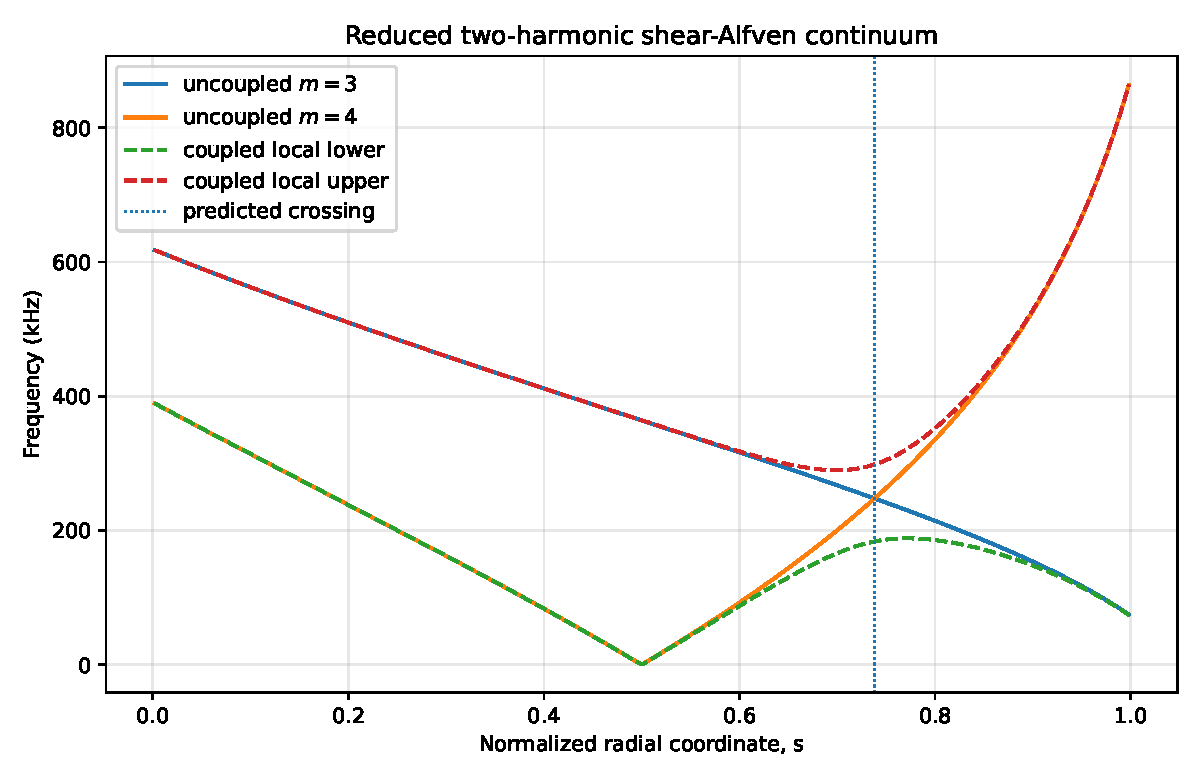
\includegraphics[width=0.88\textwidth]{figures/module4_reduced_ae_continuum.pdf}
\caption{Baseline uncoupled continuum branches and local coupled branches. The vertical line is the analytic neighboring-harmonic crossing coordinate. Frequencies are local functions of radius, not global eigenvalues.}
\label{fig:continuum_textbook}
\end{figure}

At the nearest cell center to $s_c$, the local lower and upper coupled frequencies are
\begin{equation}
f_-=\SI{183.207}{kHz},
\qquad
f_+=\SI{297.516}{kHz}.
\label{eq:baseline_gap_interval}
\end{equation}
The interval between them is a local avoided-crossing interval. It is not automatically a global gap over all radii.

\subsection{Computed global eigenfrequencies}
The frozen Python reference eigenpairs are listed in Table~\ref{tab:baseline_eigenpairs_textbook}.

\begin{table}[htbp]
\centering
\begin{tabular}{r r r}
\toprule
Mode index & Frequency (kHz) & Relative algebraic residual\\
\midrule
1 & 160.504376 & $1.38\times10^{-11}$\\
2 & 271.117830 & $6.41\times10^{-12}$\\
3 & 323.043576 & $3.99\times10^{-12}$\\
4 & 358.050072 & $5.24\times10^{-12}$\\
5 & 419.201855 & $3.25\times10^{-12}$\\
6 & 433.809373 & $4.69\times10^{-12}$\\
7 & 498.246555 & $2.90\times10^{-12}$\\
8 & 508.475762 & $2.42\times10^{-12}$\\
\bottomrule
\end{tabular}
\caption{Baseline 256-cell eigenpairs. Residuals use Eq.~\eqref{eq:relative_eigen_residual}.}
\label{tab:baseline_eigenpairs_textbook}
\end{table}

Mode 2 has frequency $\SI{271.118}{kHz}$, which lies inside the local interval in Eq.~\eqref{eq:baseline_gap_interval}. That is why it is selected for the existing representative-mode figure.

\subsection{Harmonic weights and radial localization}
For a normalized mode, define harmonic weights
\begin{align}
W_m&=\int_0^1\xi_m^2ds,\\
W_{m+1}&=\int_0^1\xi_{m+1}^2ds,
\end{align}
so $W_m+W_{m+1}=1$. Define the radial probability-like density
\begin{equation}
P(s)=\xi_m^2(s)+\xi_{m+1}^2(s).
\end{equation}
Although $P$ is not a quantum probability, its normalized integral makes it useful for reporting a centroid and spread:
\begin{align}
\bar s&=\int_0^1sP(s)ds,\\
\sigma_s&=\left[\int_0^1(s-\bar s)^2P(s)ds\right]^{1/2}.
\end{align}
Diagnostics computed directly from the frozen eigenmode CSV are shown in Table~\ref{tab:harmonic_diagnostics}.

\begin{table}[htbp]
\centering
\small
\begin{tabular}{r r r r r r}
\toprule
Mode & $W_{m=3}$ & $W_{m=4}$ & Peak $s$ & $\bar s$ & $\sigma_s$\\
\midrule
1 & 0.0069 & 0.9931 & 0.4707 & 0.4696 & 0.1258\\
2 & 0.0796 & 0.9204 & 0.2754 & 0.4294 & 0.2238\\
3 & 0.6991 & 0.3009 & 0.7324 & 0.5849 & 0.2424\\
4 & 0.1886 & 0.8114 & 0.0840 & 0.3829 & 0.2753\\
5 & 0.3089 & 0.6911 & 0.0020 & 0.4239 & 0.2581\\
6 & 0.6980 & 0.3020 & 0.4746 & 0.5018 & 0.2352\\
7 & 0.4533 & 0.5467 & 0.3730 & 0.4307 & 0.2485\\
8 & 0.5579 & 0.4421 & 0.3574 & 0.4364 & 0.2544\\
\bottomrule
\end{tabular}
\caption{Harmonic and localization diagnostics evaluated from the version-controlled 256-cell eigenvectors.}
\label{tab:harmonic_diagnostics}
\end{table}

\subsection{What the representative mode actually demonstrates}
Figure~\ref{fig:eigenmode_textbook} shows mode 2.

\begin{figure}[htbp]
\centering
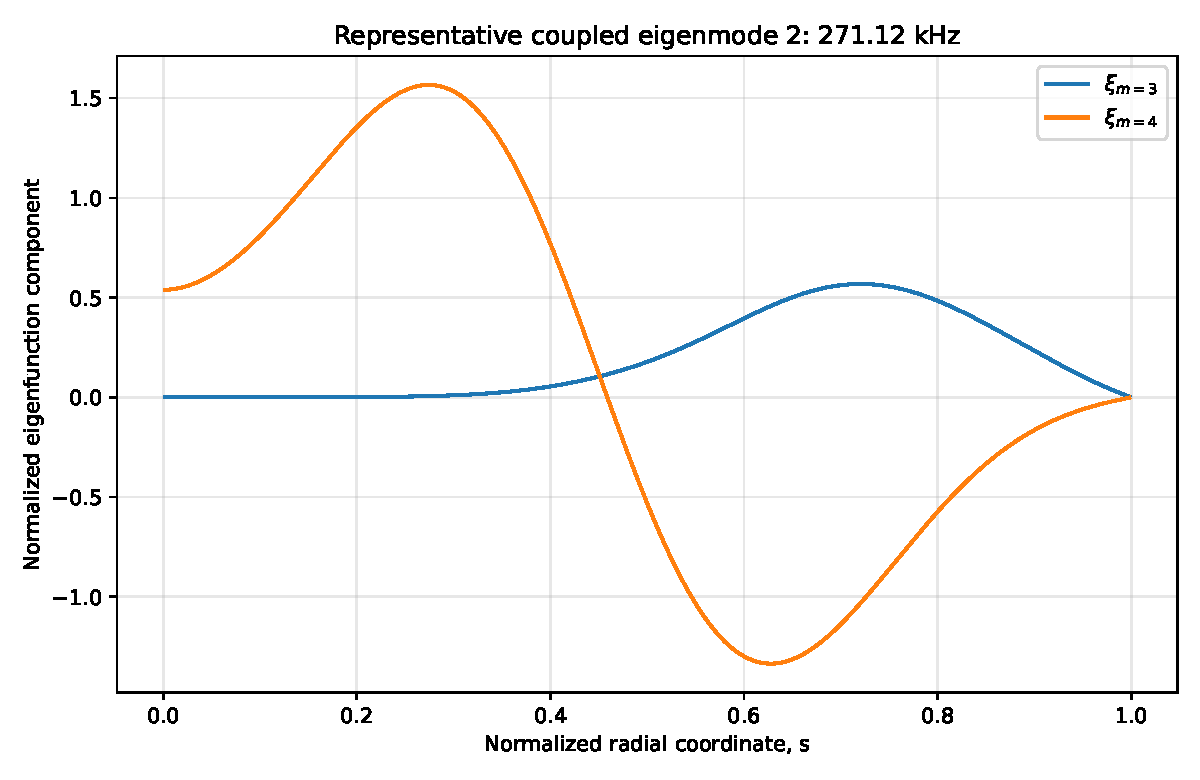
\includegraphics[width=0.86\textwidth]{figures/module4_reduced_ae_eigenmode.pdf}
\caption{Two harmonic components of mode 2, selected because its frequency is nearest the center of the local avoided-crossing interval. The mode is normalized by Eq.~\eqref{eq:benchmark_normalization}.}
\label{fig:eigenmode_textbook}
\end{figure}

The quantitative diagnostics require a careful interpretation:
\begin{itemize}[leftmargin=1.6em]
\item Mode 2 is predominantly the $m=4$ component, with $W_{m=4}\approx0.920$.
\item Its peak amplitude occurs at $s\approx0.275$, not at the analytic crossing $s_c\approx0.738$.
\item Its radial spread is broad, $\sigma_s\approx0.224$.
\item Mode 3 peaks close to $s_c$ and is more mixed, but its frequency $\SI{323.044}{kHz}$ is above the local upper branch value at the crossing cell.
\end{itemize}
Therefore, the baseline robustly demonstrates a coupled self-adjoint eigenproblem, an avoided crossing, mixed global eigenfunctions, and convergent discrete frequencies. It does \emph{not} yet demonstrate a strongly trapped, crossing-centered, realistic TAE. Calling the model a \emph{reduced coupled-harmonic benchmark with a TAE-like avoided crossing} is accurate. Calling mode 2 a validated stellarator TAE would be an overstatement.

\subsection{Why this honest limitation is useful}
A verification benchmark need not reproduce every desired physical feature. In fact, the mismatch between a local-gap frequency criterion and actual eigenfunction localization is pedagogically valuable. It shows why mode classification must use spatial structure and parameter continuation, not frequency alone. A future benchmark revision can deliberately tune $D(s)$, coupling width, profiles, or boundary conditions to generate a more clearly localized gap mode while retaining the current case as a frozen regression target.

% Module 4 section file. Included by ../module4_alfven_continuum_eigenmodes.tex.
\section{Verification, validation, convergence, and sensitivity analysis}
\label{sec:v_and_v}

\subsection{Verification versus validation}
\textbf{Verification} asks whether the equations were solved correctly. \textbf{Validation} asks whether the equations adequately represent the physical system of interest. The present project has substantial verification evidence for the reduced benchmark but no device-level validation of Module 4.

Verification activities include matrix-symmetry tests, analytic scaling tests, decoupled limits, residual checks, grid refinement, regression outputs, and Python/MATLAB parity. Validation would require comparison with experimental measurements or with trusted full-geometry eigenmode calculations using the same equilibrium and physical assumptions.

\subsection{Matrix symmetry}
The Python test checks
\begin{equation}
\frac{\|\mathbf A-\mathbf A^{\mathsf T}\|_F}{\|\mathbf A\|_F}<10^{-12},
\label{eq:symmetry_test}
\end{equation}
where $\|\cdot\|_F$ is the Frobenius norm. This test is sensitive to mismatched face coefficients, asymmetric block assembly, or an inconsistent boundary stencil.

Symmetry is necessary for the intended self-adjoint benchmark, but it is not sufficient for correctness. A symmetrically wrong matrix can still pass Eq.~\eqref{eq:symmetry_test}.

\subsection{Positive spectrum}
All requested baseline eigenvalues satisfy $\omega_j^2>0$. This is consistent with positive $D$ and locally positive-definite harmonic matrices. A stronger test could attempt a sparse Cholesky factorization or estimate the smallest eigenvalue over a broader parameter domain.

\subsection{Decoupled limit}
Set $\epsilon_c=0$. Then $\mathbf C=0$ and
\begin{equation}
\mathbf A=
\begin{bmatrix}
\mathbf K+\mathbf W_m&0\\
0&\mathbf K+\mathbf W_{m+1}
\end{bmatrix}.
\end{equation}
The global problem splits into two independent scalar eigenproblems. Locally,
\begin{equation}
\Omega_-=\min(\omega_m,\omega_{m+1}),
\qquad
\Omega_+=\max(\omega_m,\omega_{m+1}).
\end{equation}
The automated test verifies both the block structure and the local reduction. This is an important physics limit because the coupling mechanism should disappear exactly, not merely become small.

\subsection{Exact Alfv\'en scaling tests}
The tests verify:
\begin{align}
B_0\rightarrow2B_0&\quad\Rightarrow\quad f_j\rightarrow2f_j,\\
\rho(s)\rightarrow4\rho(s)&\quad\Rightarrow\quad f_j\rightarrow\frac{1}{2}f_j.
\end{align}
These transformations probe the diagonal continuum terms, the coupling, and the radial stiffness simultaneously. Failure would reveal inconsistent dimensional construction.

\subsection{Grid-refinement results}
Table~\ref{tab:grid_refinement_textbook} uses the 512-cell solution as an internal comparison rather than an exact value.

\begin{table}[htbp]
\centering
\begin{tabular}{r r r r r}
\toprule
$N$ & Mode 1 (kHz) & Relative error & Mode 2 (kHz) & Relative error\\
\midrule
64  & 160.475766 & $1.871\times10^{-4}$ & 271.034133 & $3.240\times10^{-4}$\\
128 & 160.498664 & $4.447\times10^{-5}$ & 271.101167 & $7.678\times10^{-5}$\\
256 & 160.504376 & $8.887\times10^{-6}$ & 271.117830 & $1.532\times10^{-5}$\\
512 & 160.505802 & 0 & 271.121985 & 0\\
\bottomrule
\end{tabular}
\caption{Grid refinement for the first two frequencies. Errors are relative to the 512-cell values.}
\label{tab:grid_refinement_textbook}
\end{table}

\begin{figure}[htbp]
\centering
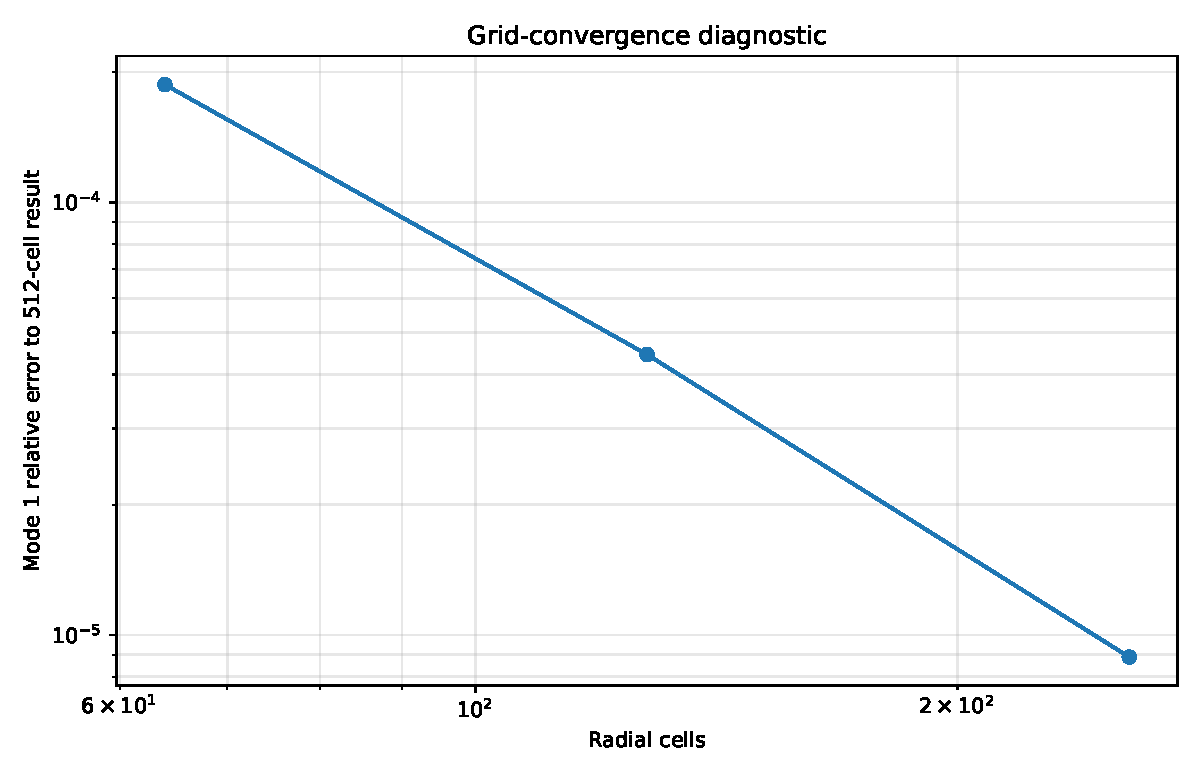
\includegraphics[width=0.82\textwidth]{figures/module4_reduced_ae_convergence.pdf}
\caption{Mode-1 frequency error relative to the 512-cell result. The trend is consistent with approximately second-order spatial behavior over the shown range.}
\label{fig:convergence_textbook}
\end{figure}

An observed order based on three grids can be estimated by
\begin{equation}
p_{\mathrm{obs}}\approx
\frac{\ln\left[(f_h-f_{h/2})/(f_{h/2}-f_{h/4})\right]}{\ln2},
\label{eq:observed_order}
\end{equation}
provided the errors have a consistent sign and the grids are in the asymptotic regime. A more rigorous study should include additional grids and Richardson extrapolation rather than treating the finest grid as exact.

\subsection{Richardson extrapolation}
If
\begin{equation}
f_h=f_*+Ch^p+O(h^{p+1}),
\end{equation}
then two successive grids with refinement ratio $r=2$ give
\begin{equation}
f_*\approx f_{h/2}+\frac{f_{h/2}-f_h}{2^p-1}.
\label{eq:richardson}
\end{equation}
This estimate separates discretization error from the arbitrary choice of finest reference. It should be added when the benchmark is promoted from a regression target to a quantified numerical standard.

\subsection{Python/MATLAB parity}
When MATLAB is available, the test criterion is
\begin{equation}
\max_j\frac{|f_j^{\mathrm{MATLAB}}-f_j^{\mathrm{Python}}|}
{f_j^{\mathrm{Python}}}<10^{-5}.
\label{eq:python_matlab_parity}
\end{equation}
The comparison also uses sign-invariant eigenvector correlation. Agreement between independently written codes reduces the likelihood of language-specific implementation error. It does not prove that both codes did not implement the same mistaken equation or interpretation.

\subsection{Regression testing}
Frozen reference outputs detect unintended changes. The Python regression tolerance for eigenfrequencies is $10^{-10}$ relative. A regression failure can result from a real defect, an intentional model change, a dependency change, or different eigensolver behavior. The appropriate response is investigation and versioning, not automatic replacement of reference data.

\subsection{Sensitivity to coupling strength}
From Eq.~\eqref{eq:gap_at_crossing_omega2}, increasing $|C|$ widens the local gap in squared frequency. Because $C\propto\epsilon_c$, the small-coupling frequency gap is approximately linear in $\epsilon_c$. Global eigenfrequencies need not shift linearly because radial envelopes and harmonic mixing change simultaneously.

A recommended scan is
\begin{equation}
\epsilon_c\in\{0,0.1,0.2,0.3,0.45,0.6,0.8\},
\end{equation}
with mode tracking by overlap. Quantities to record include local gap width, each eigenfrequency, harmonic weights, radial centroid, and overlap with the previous scan point.

\subsection{Sensitivity to radial stiffness}
Increasing $\epsilon_r$ strengthens radial coupling. Recommended diagnostics are:
\begin{equation}
\epsilon_r\in[10^{-4},10^{-2}].
\end{equation}
At very small $\epsilon_r$, envelopes may become narrow and require finer grids. At large $\epsilon_r$, boundary conditions can dominate and modes broaden across the domain. A convincing gap-localized benchmark should exhibit a parameter range in which localization near $s_c$ persists under grid refinement rather than appearing only at one tuned value.

\subsection{Sensitivity to equilibrium profiles}
The crossing position depends on $\iota_0$, $\iota_1$, and $a_\iota$. The frequency scale depends on density. Profile scans should distinguish:
\begin{itemize}[leftmargin=1.6em]
\item rigid dimensional scaling, such as multiplying all density by one factor;
\item shape changes, such as changing $a_\rho$;
\item crossing motion, such as changing $\iota_0$ or $\iota_1$;
\item loss of the crossing from the domain when $\iota_c$ falls outside the profile range.
\end{itemize}

\subsection{Additional verification tests recommended}
The next verification layer should include:
\begin{enumerate}[leftmargin=1.6em]
\item a constant-$D$, constant-potential scalar problem with an analytic mixed-boundary spectrum;
\item manufactured two-component eigenfunctions with a constructed forcing or operator coefficient;
\item discrete orthogonality checks;
\item nonuniform-grid finite-volume convergence;
\item subspace comparison for clustered modes;
\item conservation of the discrete quadratic form in a corresponding time-domain solver;
\item parameter-domain positivity tests.
\end{enumerate}

\subsection{Validation path}
A realistic validation ladder is:
\begin{enumerate}[leftmargin=1.6em]
\item compare the reduced operator with an independently derived cylindrical or large-aspect-ratio TAE model;
\item import a known axisymmetric equilibrium and compare continuum/gap estimates with a trusted code;
\item extend to a three-dimensional stellarator harmonic set and compare with a code such as CAS3D or another suitable eigenmode solver;
\item compare mode frequencies and structures with experimental diagnostics where equilibrium and density uncertainties are quantified.
\end{enumerate}
The present note stops at the verified first rung: a transparent reduced operator.

% Module 4 section file. Included by ../module4_alfven_continuum_eigenmodes.tex.
\section{Interfaces to equilibrium, kinetic drive, transport, and PINN modules}
\label{sec:interfaces}

\subsection{Module 1 to Module 4: equilibrium data contract}
A realistic fluid-MHD eigenmode solver requires far more information than the analytic benchmark. Module 1 should provide, at minimum:
\begin{itemize}[leftmargin=1.6em]
\item magnetic-surface coordinates and the mapping $\mathbf x(s,\theta,\zeta)$;
\item magnetic field $\mathbf B_0$ and magnitude $B_0$;
\item rotational transform $\iota(s)$ and magnetic shear;
\item density and pressure profiles;
\item Jacobian $\sqrt g$, metric tensors, and field-parallel derivative coefficients;
\item equilibrium current or covariant magnetic components when required;
\item plasma boundary and any vacuum or conducting-wall geometry;
\item Fourier conventions, field-period convention, and coordinate normalization.
\end{itemize}
The reduced benchmark uses only $R_0$, constant $B_0$, $\rho(s)$, and $\iota(s)$. It should therefore be regarded as an interface prototype, not a complete consumer of Module 1 output.

\subsection{Module 4 outputs needed by Module 5}
A kinetic energetic-particle calculation needs more than a scalar frequency. The desired Module 4 output for each mode includes
\begin{equation}
\mathcal M_j=
\left\{
\omega_{r,j},
\boldsymbol\xi_j(\mathbf x),
\delta\mathbf B_j(\mathbf x),
\delta\mathbf E_j(\mathbf x),
\{m,n\}\text{ spectrum},
\text{normalization},
\text{continuum relation}
\right\}.
\end{equation}
The fields follow from the displacement in ideal MHD:
\begin{align}
\delta\mathbf B_j&=\nabla\times(\boldsymbol\xi_j\times\mathbf B_0),\\
\delta\mathbf E_j&=-\mathbf v_{1,j}\times\mathbf B_0
=i\omega_{r,j}\boldsymbol\xi_j\times\mathbf B_0
\end{align}
for the $e^{-i\omega t}$ convention. Module 5 then evaluates resonance conditions and power transfer along energetic-particle orbits.

The current benchmark outputs only reduced radial envelopes, not full three-dimensional fields. It can validate an eigenvalue PINN but cannot yet support a quantitative orbit-wave coupling integral.

\subsection{Kinetic resonance condition}
A general orbit resonance has the form
\begin{equation}
\omega_r-n\Omega_\zeta-\ell\Omega_\theta-p\Omega_b\approx0,
\label{eq:general_orbit_resonance}
\end{equation}
where $\Omega_\zeta$, $\Omega_\theta$, and $\Omega_b$ denote toroidal, poloidal, and bounce or transit frequencies according to the orbit representation, and $\ell,p$ are integers. The exact notation varies between passing and trapped particles and between coordinate systems.

The kinetic module computes a contribution to the complex frequency,
\begin{equation}
\omega=\omega_r+i\gamma,
\end{equation}
with
\begin{equation}
\gamma_{\mathrm{net}}=
\gamma_{\mathrm{EP}}
-\gamma_{\mathrm{continuum}}
-\gamma_{\mathrm{Landau}}
-\gamma_{\mathrm{FLR}}
-\gamma_{\mathrm{collisional}}
-\cdots.
\end{equation}
Module 4 supplies the real baseline mode. Module 5 supplies drive and damping corrections or a more complete non-self-adjoint eigenproblem.

\subsection{Module 4 to Module 6: transport closure}
If a mode is unstable, it can perturb energetic-particle invariants and cause phase-space transport. A reduced transport model may use a mode-dependent diffusion coefficient
\begin{equation}
D_{\mathrm{AE}}=D_{\mathrm{AE}}
\left(|A_j|^2,\omega_j,\gamma_j,\boldsymbol\xi_j,f_f,\text{resonances}\right).
\end{equation}
The linear Module 4 eigenproblem does not determine amplitude $A_j$. A saturation model, nonlinear simulation, or empirical closure is required before Module 6 can compute a physical transport rate.

\subsection{Module 9 eigenvalue PINN target}
The conventional benchmark supplies a well-defined target for an eigenvalue PINN. A neural network may represent
\begin{equation}
\widehat{\boldsymbol\xi}(s;\boldsymbol\theta)
=\begin{bmatrix}
\widehat\xi_m(s;\boldsymbol\theta)\\
\widehat\xi_{m+1}(s;\boldsymbol\theta)
\end{bmatrix},
\end{equation}
with trainable parameters $\boldsymbol\theta$ and a trainable or inferred $\widehat\omega^2$. The differential residual is
\begin{equation}
\mathbf r_{\mathrm{PDE}}(s)=
-\frac{d}{ds}\left(D\frac{d\widehat{\boldsymbol\xi}}{ds}\right)
+\mathbf H_{\mathrm{loc}}\widehat{\boldsymbol\xi}
-\widehat\omega^2\widehat{\boldsymbol\xi}.
\end{equation}
A schematic loss is
\begin{equation}
\mathcal L=
\lambda_r\langle\|\mathbf r_{\mathrm{PDE}}\|^2\rangle
+\lambda_{\mathrm{BC}}\mathcal L_{\mathrm{BC}}
+\lambda_N\left(\widehat{\mathcal N}-1\right)^2
+\lambda_O\mathcal L_{\mathrm{orth}}
+\lambda_D\mathcal L_{\mathrm{data}}.
\label{eq:eigen_pinn_loss}
\end{equation}
The normalization term prevents the trivial zero solution. For multiple modes, orthogonality or deflation is required. Boundary conditions can be imposed softly through loss terms or exactly through a trial-function transformation.

\subsection{PINN failure modes specific to eigenproblems}
An eigenvalue PINN may:
\begin{itemize}[leftmargin=1.6em]
\item converge to the zero function if normalization is weak;
\item repeatedly learn the lowest mode instead of higher modes;
\item satisfy pointwise residuals poorly near sharp layers;
\item return a plausible eigenvalue with an incorrect eigenfunction;
\item mix nearly degenerate modes differently from the reference;
\item minimize a biased collocation loss while violating the variational structure;
\item learn a discretized continuum state rather than the intended global mode.
\end{itemize}
Success criteria must include frequency error, residual, boundary error, normalization, eigenfunction correlation, harmonic weights, orthogonality, and performance under parameter variation.

\subsection{Variational neural alternative}
Instead of minimizing the strong-form residual, one may minimize the Rayleigh quotient
\begin{equation}
\widehat\omega^2(\boldsymbol\theta)
=\frac{\mathcal E[\widehat{\boldsymbol\xi}]}
{\mathcal N[\widehat{\boldsymbol\xi}]}
\end{equation}
subject to boundary conditions and orthogonality to previously found modes. This respects self-adjoint structure and can reduce the order of derivatives appearing in the loss. However, it can still collapse to the lowest eigenmode and requires accurate quadrature.

\subsection{Language-neutral output contract}
The benchmark writes:
\begin{itemize}[leftmargin=1.6em]
\item \texttt{profiles\_and\_continuum.csv}: $s$, density, transform, $v_A$, uncoupled branches, coupling, and local coupled branches;
\item \texttt{eigenvalues.csv}: mode index, $\omega^2$, $\omega$, $f$, and residual;
\item \texttt{eigenmodes.csv}: both harmonic envelopes for every requested mode;
\item \texttt{convergence.csv}: grid-refinement frequencies and errors;
\item \texttt{metadata.json}: crossing, local gap, boundary conditions, normalization, and solver identity;
\item PDF and PNG visualizations.
\end{itemize}
These products permit code parity, regression testing, and machine-learning ingestion without coupling downstream tools to Python-specific or MATLAB-specific binary formats.

\subsection{Fidelity progression}
A defensible development sequence is
\begin{equation}
\begin{aligned}
\text{two harmonics}
&\rightarrow \text{many harmonics}
\rightarrow \text{equilibrium-derived coefficients}\\
&\rightarrow \text{3D stellarator coupling}
\rightarrow \text{kinetic corrections}\\
&\rightarrow \text{surrogates and digital twin}.
\end{aligned}
\end{equation}
At each stage, the lower-fidelity benchmark should remain frozen. Higher fidelity should add new cases and tests rather than silently changing the meaning of an established reference.

% Module 4 section file. Included by ../module4_alfven_continuum_eigenmodes.tex.
\section{Worked examples}
\label{sec:worked_examples}

\subsection{Example 1: calculate an Alfv\'en speed and frequency}
Let
\begin{equation}
B_0=\SI{2.5}{T},
\qquad
\rho=3.3\times10^{-8}\ \mathrm{kg\,m^{-3}}.
\end{equation}
Then
\begin{align}
v_A
&=\frac{B_0}{\sqrt{\mu_0\rho}}\\
&=\frac{2.5}{\sqrt{(4\pi\times10^{-7})(3.3\times10^{-8})}}\\
&\approx1.228\times10^7\ \mathrm{m\,s^{-1}}.
\end{align}
Suppose $R_0=\SI{3}{m}$, $n=2$, $m=4$, and $\iota=0.50$. Then
\begin{equation}
n-m\iota=2-4(0.50)=0.
\end{equation}
This harmonic is at a rational surface and the reduced uncoupled frequency is zero. If instead $\iota=0.45$,
\begin{equation}
|n-m\iota|=|2-1.8|=0.2,
\end{equation}
so
\begin{align}
\omega_m&=0.2\frac{v_A}{R_0}
\approx0.2\frac{1.228\times10^7}{3}
\approx8.19\times10^5\ \mathrm{s^{-1}},\\
f_m&=\frac{\omega_m}{2\pi}\approx\SI{130}{kHz}.
\end{align}
This example shows that the dimensional scale $v_A/R_0$ is multiplied by a potentially small field-line phase factor $|n-m\iota|$.

\subsection{Example 2: locate the neighboring-harmonic crossing}
Take $n=2$, $m=3$, $\iota_0=0.35$, $\iota_1=0.65$, and $a_\iota=1$. The crossing transform is
\begin{equation}
\iota_c=\frac{2n}{2m+1}=\frac{4}{7}=0.5714286.
\end{equation}
The inverse profile gives
\begin{equation}
s_c=\frac{0.5714286-0.35}{0.65-0.35}=0.7380952.
\end{equation}
Check the two signed factors:
\begin{align}
n-m\iota_c&=2-3\left(\frac{4}{7}\right)=\frac{2}{7},\\
n-(m+1)\iota_c&=2-4\left(\frac{4}{7}\right)=-\frac{2}{7}.
\end{align}
They are equal and opposite, as required.

\subsection{Example 3: compute the local avoided-crossing gap}
Suppose the uncoupled crossing angular frequency is
\begin{equation}
\omega_c=1.50\times10^6\ \mathrm{s^{-1}}
\end{equation}
and the coupling is
\begin{equation}
C=0.20\omega_c^2.
\end{equation}
At the crossing,
\begin{align}
\Omega_-&=\omega_c\sqrt{1-0.20}=0.8944\omega_c,\\
\Omega_+&=\omega_c\sqrt{1+0.20}=1.0954\omega_c.
\end{align}
Therefore
\begin{equation}
\Delta\omega=(1.0954-0.8944)\omega_c=0.2010\omega_c.
\end{equation}
The small-coupling estimate gives
\begin{equation}
\Delta\omega\approx\frac{C}{\omega_c}=0.20\omega_c,
\end{equation}
which is accurate here to about one-half percent.

\subsection{Example 4: harmonic mixing away from and at the crossing}
Let $a-b=4C$. Then
\begin{equation}
\tan2\alpha=\frac{2C}{a-b}=\frac{1}{2},
\end{equation}
so
\begin{equation}
2\alpha\approx26.565^\circ,
\qquad
\alpha\approx13.283^\circ.
\end{equation}
The lower branch has weights approximately
\begin{equation}
\cos^2\alpha\approx0.947,
\qquad
\sin^2\alpha\approx0.053.
\end{equation}
It remains mostly one harmonic. At $a=b$, $\alpha=45^\circ$ and both weights are $0.5$. Equal mixing is therefore a localized feature of the crossing region unless coupling is very strong.

\subsection{Example 5: derive one interior finite-volume row}
Let $h=0.1$, $D_{i-1/2}=2.0\times10^9\ \mathrm{s^{-2}}$, and $D_{i+1/2}=3.0\times10^9\ \mathrm{s^{-2}}$. From Eq.~\eqref{eq:interior_stencil},
\begin{align}
K_{i,i-1}&=-\frac{2.0\times10^9}{0.1^2}=-2.0\times10^{11}\ \mathrm{s^{-2}},\\
K_{i,i}&=\frac{2.0\times10^9+3.0\times10^9}{0.1^2}=5.0\times10^{11}\ \mathrm{s^{-2}},\\
K_{i,i+1}&=-\frac{3.0\times10^9}{0.1^2}=-3.0\times10^{11}\ \mathrm{s^{-2}}.
\end{align}
The row sum is zero because an interior constant function has zero gradient. At the edge, the Dirichlet penalty makes the row sum nonzero and removes the constant null mode.

\subsection{Example 6: normalize a discrete two-harmonic mode}
Suppose $N=4$, so $h=0.25$, and an unnormalized vector is
\begin{equation}
\mathbf x=
\begin{bmatrix}
1&2&1&0&\;0&1&1&0
\end{bmatrix}^{\mathsf T}.
\end{equation}
Its Euclidean squared norm is
\begin{equation}
\mathbf x^{\mathsf T}\mathbf x=1+4+1+0+0+1+1+0=8.
\end{equation}
The grid-weighted norm is
\begin{equation}
h\mathbf x^{\mathsf T}\mathbf x=0.25(8)=2.
\end{equation}
Therefore the normalized vector is
\begin{equation}
\mathbf x_N=\frac{\mathbf x}{\sqrt2}.
\end{equation}
Using only Euclidean normalization would produce an integral norm of $h=0.25$ rather than one.

\subsection{Example 7: separate residual error from discretization error}
Assume a 128-cell calculation gives $f_{128}=\SI{271.101167}{kHz}$ with residual $10^{-12}$, while a 256-cell calculation gives $f_{256}=\SI{271.117830}{kHz}$ with the same residual. The relative difference is
\begin{equation}
\frac{|f_{256}-f_{128}|}{f_{256}}
\approx6.15\times10^{-5}.
\end{equation}
The eigensolver has solved each discrete matrix extremely accurately, but the spatial discretization still shifts the frequency by tens of parts per million. A smaller algebraic residual would not remove this grid error.

\subsection{Example 8: test exact magnetic-field scaling}
Let a reference eigenfrequency be
\begin{equation}
f_1(B_0=\SI{2.5}{T})=\SI{160.504376}{kHz}.
\end{equation}
If the field is doubled to \SI{5.0}{T}, the benchmark predicts exactly
\begin{equation}
f_1=2(160.504376)=\SI{321.008752}{kHz}
\end{equation}
up to numerical roundoff, because every matrix coefficient scales as $B_0^2$.

\subsection{Example 9: determine whether a frequency criterion is sufficient}
Mode 2 has $f_2=\SI{271.118}{kHz}$, inside the local crossing-cell interval $[183.207,297.516]\ \mathrm{kHz}$. However, its peak is at $s\approx0.275$, its centroid is $\bar s\approx0.429$, and $W_{m=4}\approx0.920$. Therefore:
\begin{equation}
\text{frequency in local interval}
\not\Rightarrow
\text{strong localization at }s_c.
\end{equation}
The correct conclusion is that the mode is useful for coupled-harmonic verification, not that frequency alone proves a trapped TAE.

\subsection{Example 10: construct a PINN trial function satisfying both boundaries}
For one component, let a neural network output $N_\theta(s)$. A trial function
\begin{equation}
\widehat\xi(s)=(1-s)N_\theta(s)
\end{equation}
satisfies the edge Dirichlet condition but not necessarily the axis Neumann condition. To satisfy both exactly, use a function of $s^2$:
\begin{equation}
\boxed{\widehat\xi(s)=(1-s^2)N_\theta(s^2).}
\end{equation}
At $s=1$, $\widehat\xi=0$. At $s=0$, every term in $d\widehat\xi/ds$ contains a factor of $s$, so $\widehat\xi'(0)=0$. The construction must be applied to both harmonic components, followed by normalization and mode-selection constraints.

% Module 4 section file. Included by ../module4_alfven_continuum_eigenmodes.tex.
\section{Common misconceptions and failure modes}
\label{sec:misconceptions}

\subsection{``Kinetic MHD should not use fluid MHD''}
Incorrect. Kinetic MHD is commonly a hybrid theory. The bulk plasma can be described by MHD while energetic or resonant populations are treated kinetically. Module 4 supplies the fluid restoring-force structure; Module 5 supplies kinetic energy exchange.

\subsection{``Every particle moves at the fluid velocity''}
Incorrect. Fluid velocity is a velocity moment of a distribution function. It is not assigned to every particle. A Maxwellian or non-Maxwellian distribution contains many individual velocities even when the bulk velocity is zero.

\subsection{``The Alfv\'en continuum is one curve''}
Usually incorrect. Each Fourier harmonic and wave family can produce a branch, and three-dimensional coupling produces many interacting branches. A plotted pair in the benchmark is a deliberately truncated subset.

\subsection{``A rational surface always means an instability''}
Incorrect. A rational surface means a selected Fourier phase has $k_\parallel=0$ under the adopted approximation. Stability depends on the full energy balance, gradients, currents, pressure, coupling, and nonideal effects.

\subsection{``A local gap automatically contains a global TAE''}
Incorrect. A local avoided crossing is obtained by diagonalizing a small matrix independently at each radius. A global mode requires a radial differential solution and appropriate boundary conditions. It may fail to localize or may intersect another continuum branch elsewhere.

\subsection{``Any eigenfrequency in the gap proves the mode is gap localized''}
Incorrect. The baseline mode-2 result is a direct counterexample to using frequency alone. Harmonic weights, radial localization, convergence, and continuum intersections must also be examined.

\subsection{``The absolute sign of an eigenvector is physical''}
Incorrect for a homogeneous linear eigenproblem. $\mathbf x$ and $-\mathbf x$ represent the same real mode. For complex vectors, an arbitrary global phase is also unphysical.

\subsection{``Small residual means correct physics''}
Incorrect. A residual tests the discrete algebraic equation. Model-form error, incorrect coefficients, inadequate geometry, and spatial discretization error can remain large.

\subsection{``Python--MATLAB agreement validates the plasma model''}
Incorrect. Cross-code parity is strong implementation verification, but both codes may solve the same reduced or mistaken model. Validation requires comparison with trusted physical calculations or experiment.

\subsection{``A finite matrix literally contains a mathematical continuum''}
Incorrect. A finite matrix contains discrete eigenvalues. It approximates a continuum through a resolution-dependent collection of states. Grid behavior is part of the physical interpretation.

\subsection{``The edge Dirichlet condition is universal''}
Incorrect. It is a benchmark choice. Real modes may require plasma-vacuum matching, conducting-wall conditions, radiative conditions, or regularity constraints in variables different from the reduced envelope.

\subsection{``The minor radius in the JSON determines the radial derivative''}
Not in the current implementation. The operator differentiates with respect to dimensionless $s$ and uses $D$ with units of frequency squared. The stored minor radius is metadata for future models.

\subsection{``The two-harmonic coupling coefficient is a measured toroidicity coefficient''}
Incorrect. $C(s)$ is a prescribed Gaussian surrogate. It reproduces the mathematics of avoided crossing and harmonic mixing but is not extracted from a VMEC, DESC, or other equilibrium.

\subsection{``The lowest sorted mode remains the same physical mode during a scan''}
Not necessarily. Global avoided crossings can exchange eigenfunction character. Mode tracking should use overlaps and subspace methods.

\subsection{``Clipping negative eigenvalues before the square root is harmless''}
Potentially dangerous. Tiny negative values caused solely by floating-point roundoff in a locally positive expression may be clipped defensively. A negative global eigenvalue from the eigensolver must be investigated because it may indicate instability or a defective operator.

\subsection{``A larger neural network guarantees a better eigenvalue PINN''}
Incorrect. Eigenvalue PINNs have structural difficulties: the zero solution, mode collapse, orthogonality, sharp layers, spectral bias, and loss imbalance. Architecture size alone does not solve these problems.

\subsection{Numerical failure modes checklist}
Before accepting a result, check for:
\begin{itemize}[leftmargin=1.6em]
\item inconsistent Fourier signs between equilibrium, solver, and diagnostic code;
\item confusion between angular frequency $\omega$ and ordinary frequency $f$;
\item confusion between mass density and number density;
\item missing factor $2\pi$ in frequency conversion;
\item wrong half-cell distance at the edge boundary;
\item face coefficients evaluated inconsistently on opposite matrix rows;
\item Euclidean normalization mistaken for grid-weight normalization;
\item sorted-index mode matching across a crossing;
\item unresolved radial localization or continuum layers;
\item reference files regenerated without documenting the reason;
\item physical claims exceeding the fidelity stated in metadata.
\end{itemize}

% Module 4 section file. Included by ../module4_alfven_continuum_eigenmodes.tex.
\section{Exercises and computational laboratories}
\label{sec:exercises}

\subsection{Conceptual exercises}
\begin{enumerate}[leftmargin=1.8em]
\item Explain in words why a transverse displacement that is constant along a uniform field produces no shear-Alfv\'en restoring force.
\item Distinguish magnetic pressure from magnetic tension using Eq.~\eqref{eq:magnetic_pressure_tension}.
\item Explain why a fluid-MHD eigenmode is a legitimate component of a kinetic-MHD model.
\item Explain why $\omega_A(s)$ forms a continuum when $s$ is continuous.
\item Distinguish a rational surface, a continuum-resonant surface, and a neighboring-harmonic crossing surface.
\item Explain why a local avoided crossing does not prove the existence of a global gap mode.
\item Explain why mode amplitude is undetermined in a homogeneous linear eigenproblem.
\item Explain the difference between verification and validation using the current benchmark as an example.
\end{enumerate}

\subsection{Derivation exercises}
\begin{enumerate}[leftmargin=1.8em]
\item Starting from Eqs.~\eqref{eq:mhd_induction} and \eqref{eq:v_xi}, derive Eq.~\eqref{eq:b1_xi}.
\item Starting from the adiabatic pressure equation, derive Eq.~\eqref{eq:p1_xi}.
\item Repeat the uniform shear-Alfv\'en derivation for displacement in the $y$ direction.
\item Show explicitly that the uniform shear-Alfv\'en wave has equal cycle-averaged kinetic and magnetic energy.
\item Derive Eq.~\eqref{eq:kparallel_benchmark} from the stated Fourier convention and field-line pitch, carefully documenting the sign convention.
\item Derive the logarithmic continuum slope in Eq.~\eqref{eq:continuum_log_slope}.
\item Diagonalize Eq.~\eqref{eq:generic_two_mode_matrix} and derive both eigenvalues and the mixing-angle relation.
\item Derive the crossing transform and crossing frequency in Eqs.~\eqref{eq:tae_crossing_iota}--\eqref{eq:tae_gap_center}.
\item Derive the Euler--Lagrange equations from Eqs.~\eqref{eq:reduced_energy}--\eqref{eq:reduced_norm}.
\item Prove the discrete positivity identity in Eq.~\eqref{eq:discrete_K_positive}.
\end{enumerate}

\subsection{Numerical exercises}
\begin{enumerate}[leftmargin=1.8em]
\item Reproduce the baseline density, transform, Alfv\'en speed, and uncoupled continuum arrays directly from the JSON file without calling the project solver.
\item Verify the crossing location numerically and compare the exact $s_c$ with the nearest cell center for $N=64,128,256,512$.
\item Set $\epsilon_c=0$ and verify that the two block families can be solved independently.
\item Scan $B_0$ and confirm that every frequency is linear in $B_0$ while normalized eigenvectors remain unchanged to numerical precision.
\item Scan a uniform density multiplier and confirm the inverse-square-root scaling.
\item Compute the observed convergence order for modes 1--4 using at least four grids and Richardson extrapolation.
\item Calculate the discrete orthogonality matrix $h\mathbf X^{\mathsf T}\mathbf X$.
\item Reproduce Table~\ref{tab:harmonic_diagnostics} from the eigenmode CSV.
\item Track modes through a coupling scan using maximum eigenvector overlap. Compare with sorted-index tracking.
\item Replace the arithmetic face average by a harmonic average and determine the convergence difference for the smooth baseline coefficient.
\end{enumerate}

\subsection{Model-development laboratories}
\begin{enumerate}[leftmargin=1.8em]
\item Tune $\epsilon_c$, $w_c$, and $\epsilon_r$ to produce a mode whose frequency lies in the local gap and whose radial density peaks near $s_c$. Preserve the original case and create a separately versioned case.
\item Generalize the operator to $M$ harmonics with a sparse coupling graph. Verify symmetry and the decoupled limit for every edge of the graph.
\item Add a nonuniform mass matrix $\mathbf M$ and solve $\mathbf A\mathbf x=\omega^2\mathbf M\mathbf x$. Define the correct normalization and residual.
\item Construct a cylindrical analytic benchmark with constant $D$ and constant potential so that mixed-boundary eigenvalues are known exactly.
\item Implement a nonuniform radial grid and derive face distances and cell widths carefully.
\item Create an eigenvalue PINN using the exact boundary-satisfying trial function from Worked Example 10. Compare strong-form and variational losses.
\item Train multiple neural modes using orthogonality constraints. Test whether the network repeatedly collapses to the lowest mode.
\item Import an equilibrium-derived $\iota(s)$ and density profile while retaining the surrogate coupling. Quantify which changes are simple rescalings and which alter mode structure.
\item Replace the surrogate coupling with coefficients derived from a controlled large-aspect-ratio toroidal model.
\item Design a validation case against a trusted external eigenmode code, including equilibrium conversion, harmonic convention, normalization, and uncertainty accounting.
\end{enumerate}

\section{Chapter summary}
\label{sec:summary}

\begin{physicsbox}
\textbf{Physical chain.}
\begin{equation*}
\begin{aligned}
\text{magnetic tension}
&\rightarrow \omega=|k_\parallel|v_A
\rightarrow \omega_m(s)\\
&\rightarrow \text{Alfv\'en continuum}
\rightarrow \text{geometric harmonic coupling}\\
&\rightarrow \text{spectral gaps}
\rightarrow \text{global eigenmodes}.
\end{aligned}
\end{equation*}
\end{physicsbox}

The shear-Alfv\'en wave is a transverse fluid-MHD oscillation restored mainly by magnetic tension. In a uniform medium it satisfies
\begin{equation}
\omega^2=k_\parallel^2v_A^2,
\qquad
v_A=\frac{B_0}{\sqrt{\mu_0\rho_0}}.
\end{equation}
In a toroidal plasma, field-line pitch and density vary across magnetic surfaces. For the benchmark convention,
\begin{equation}
k_{\parallel,m}=\frac{n-m\iota}{R_0},
\end{equation}
so each harmonic has a radially varying local continuum branch.

Toroidal and three-dimensional geometry couples Fourier harmonics. A symmetric two-mode matrix produces avoided crossing, harmonic mixing, and a local gap. Neighboring harmonics $m$ and $m+1$ cross at
\begin{equation}
\iota_c=\frac{2n}{2m+1}.
\end{equation}
A local gap alone does not establish a global eigenmode. Radial derivatives and boundary conditions must be solved.

The project's executable benchmark uses two coupled radial envelopes:
\begin{equation}
-\frac{d}{ds}\left(D\frac{d\boldsymbol\xi}{ds}\right)
+\mathbf H_{\mathrm{loc}}\boldsymbol\xi
=\omega^2\boldsymbol\xi.
\end{equation}
It follows from a positive quadratic functional and is self-adjoint under zero axis flux and zero edge value. A cell-centered finite-volume discretization produces a real symmetric sparse matrix.

The baseline solver is strongly verified as a reduced numerical benchmark: it passes symmetry, decoupling, exact Alfv\'en scaling, residual, regression, and grid-refinement tests; Python reference tests pass, and MATLAB parity is defined for environments with MATLAB. The frozen output demonstrates coupled branches and convergent mixed-harmonic eigenmodes.

The baseline should not be overinterpreted. Mode 2 lies within the local crossing-cell interval but is not strongly localized at the crossing and is dominated by one harmonic. The current result is therefore not a validated predictive stellarator TAE. It is a transparent conventional target for the next stages: many-harmonic geometry, equilibrium-derived coefficients, kinetic drive and damping, and eigenvalue PINNs.

\section{Minimum interview-level explanation}
A concise but technically accurate explanation is:

\begin{overviewbox}
A shear-Alfv\'en wave bends magnetic field lines, and magnetic tension restores them. Its local frequency is approximately $\omega_A=|k_\parallel|v_A$. In a toroidal plasma, rotational transform, magnetic geometry, and density vary across flux surfaces, so the local Alfv\'en frequency forms a continuum. Toroidal or stellarator geometry couples Fourier harmonics and opens gaps at avoided crossings. Global Alfv\'en eigenmodes can form through radial coupling and boundary conditions, sometimes inside those gaps. Module 4 solves a verified reduced fluid-MHD eigenproblem for that structure. Module 5 then determines whether energetic particles drive or damp the mode through kinetic resonances.
\end{overviewbox}

\section{Completion checklist for the reader}
A reader is prepared to move to Module 5 when they can answer all of the following without relying on memorized phrases:
\begin{itemize}[leftmargin=1.6em]
\item What physical force restores a shear-Alfv\'en wave?
\item Why is $v_A$ proportional to $B$ and inversely proportional to $\sqrt\rho$?
\item How is $k_\parallel$ obtained from $(m,n,\iota)$ under a stated convention?
\item Why does radial nonuniformity create a continuum?
\item What is the difference between a local continuum branch and a global eigenmode?
\item How does a $2\times2$ coupling matrix open a gap?
\item Why is a mode frequency insufficient for classifying a TAE?
\item Why is the reduced operator self-adjoint?
\item How are the axis and edge boundary conditions discretized?
\item What do residual, grid convergence, and code parity each establish?
\item Which information must Module 4 pass to a kinetic resonance calculation?
\end{itemize}

% Module 4 section file. Included by ../module4_alfven_continuum_eigenmodes.tex.
\section{References and further reading}
\label{sec:references}

The references below include foundational ideal-MHD, Alfv\'en-wave, continuum, eigenmode, stellarator, and numerical sources. They do not imply that the reduced benchmark implements the full models in those publications.

\begin{enumerate}[leftmargin=1.8em]
\item H. Alfv\'en, ``Existence of electromagnetic-hydrodynamic waves,'' \emph{Nature} \textbf{150}, 405--406 (1942). The original introduction of what are now called Alfv\'en waves.

\item J. P. Freidberg, \emph{Ideal Magnetohydrodynamics}, Plenum Press, New York (1987). Standard derivations of ideal-MHD equilibrium, linear stability, and the energy principle.

\item J. P. Freidberg, \emph{Plasma Physics and Fusion Energy}, Cambridge University Press (2007). Accessible treatment of magnetic confinement and MHD waves.

\item J. P. Goedbloed, R. Keppens, and S. Poedts, \emph{Advanced Magnetohydrodynamics}, Cambridge University Press (2010). Comprehensive spectral theory and MHD continua.

\item J. P. Goedbloed and S. Poedts, \emph{Principles of Magnetohydrodynamics}, Cambridge University Press (2004). Mathematical structure of ideal and resistive MHD.

\item I. B. Bernstein, E. A. Frieman, M. D. Kruskal, and R. M. Kulsrud, ``An energy principle for hydromagnetic stability problems,'' \emph{Proceedings of the Royal Society A} \textbf{244}, 17--40 (1958). Foundational ideal-MHD energy principle.

\item C. Z. Cheng, L. Chen, and M. S. Chance, ``High-$n$ ideal and resistive shear Alfv\'en waves in tokamaks,'' \emph{Annals of Physics} \textbf{161}, 21--47 (1985), doi:10.1016/0003-4916(85)90335-5.

\item G. Y. Fu and J. W. Van Dam, ``Excitation of the toroidicity-induced shear Alfv\'en eigenmode by fusion alpha particles in an ignited tokamak,'' \emph{Physics of Fluids B} \textbf{1}, 1949--1952 (1989).

\item F. Zonca and L. Chen, ``Theory of toroidal Alfv\'en modes excited by energetic particles in tokamaks,'' \emph{Physics of Plasmas} \textbf{3}, 323--343 (1996), doi:10.1063/1.871857.

\item L. Chen and F. Zonca, ``Physics of Alfv\'en waves and energetic particles in burning plasmas,'' \emph{Reviews of Modern Physics} \textbf{88}, 015008 (2016), doi:10.1103/RevModPhys.88.015008.

\item W. W. Heidbrink, ``Basic physics of Alfv\'en instabilities driven by energetic particles in toroidally confined plasmas,'' \emph{Physics of Plasmas} \textbf{15}, 055501 (2008), doi:10.1063/1.2838239.

\item N. N. Gorelenkov, ``Revisiting eigenmode interaction with the Alfv\'en continuum,'' \emph{Physical Review Letters} \textbf{95}, 265003 (2005), doi:10.1103/PhysRevLett.95.265003.

\item D. A. Spong, E. D'Azevedo, and Y. Todo, ``Clustered frequency analysis of shear Alfv\'en modes in stellarators,'' and related stellarator Alfv\'en-eigenmode literature. Consult device-specific publications for the exact operator and coupling conventions used in each code.

\item J. Varela, A. Shimizu, D. A. Spong, L. Garcia, and Y. Ghai, ``Study of the Alfv\'en eigenmodes stability in CFQS plasma using a Landau closure model,'' \emph{Nuclear Fusion} \textbf{61}, 026023 (2021), doi:10.1088/1741-4326/abd072.

\item S. P. Hirshman and J. C. Whitson, ``Steepest-descent moment method for three-dimensional magnetohydrodynamic equilibria,'' \emph{Physics of Fluids} \textbf{26}, 3553--3568 (1983). Foundation of the VMEC equilibrium method that can supply geometry to later Module 4 fidelity levels.

\item R. LeVeque, \emph{Finite Volume Methods for Hyperbolic Problems}, Cambridge University Press (2002). General finite-volume principles; the benchmark applies the conservative flux idea to a self-adjoint radial operator rather than a hyperbolic conservation law.

\item Y. Saad, \emph{Numerical Methods for Large Eigenvalue Problems}, revised edition, Society for Industrial and Applied Mathematics (2011). Krylov-subspace and sparse eigenvalue methods.

\item G. H. Golub and C. F. Van Loan, \emph{Matrix Computations}, fourth edition, Johns Hopkins University Press (2013). Symmetric eigenproblems, residuals, conditioning, and subspace methods.

\item A. Quarteroni, R. Sacco, and F. Saleri, \emph{Numerical Mathematics}, second edition, Springer (2007). Discretization error, eigenproblems, and numerical verification concepts.

\item P. J. Schmid, ``Dynamic mode decomposition of numerical and experimental data,'' \emph{Journal of Fluid Mechanics} \textbf{656}, 5--28 (2010). Not an MHD eigenmode solver, but useful for distinguishing operator eigenanalysis from data-driven modal decompositions.
\end{enumerate}

\begin{notebox}
\textbf{Reference discipline.} Before comparing formulas between sources, check the Fourier phase, sign of toroidal angle, definition of $n$, definition of rotational transform or safety factor, use of angular versus ordinary frequency, and normalization of magnetic flux. Many apparent contradictions are convention differences.
\end{notebox}


\end{document}
